\documentclass[12pt]{article}
\usepackage[english]{babel}
\usepackage{lipsum}
\usepackage[square, numbers]{natbib}
\bibliographystyle{plainurl}
\usepackage{url}
\usepackage[utf8x]{inputenc}
\usepackage{amsmath}
\usepackage{graphicx}
\graphicspath{{images/}}
\usepackage{parskip}
\usepackage{fancyhdr}
\usepackage{vmargin}
\usepackage{hyperref}
\usepackage{todonotes}
\usepackage{textcomp}
\usepackage{float}
\usepackage{listings}
\usepackage{enumitem}
\usepackage{color} %red, green, blue, yellow, cyan, magenta, black, white
\definecolor{mygreen}{RGB}{28,172,0} % color values Red, Green, Blue
\definecolor{mylilas}{RGB}{170,55,241}
\setmarginsrb{2 cm}{2.5 cm}{2 cm}{2.5 cm}{1 cm}{1 cm}{1 cm}{1 cm}

\title{Signal Processing for Radar Applications}
\author{A. Scharf}	
\date{\today}

\makeatletter
\let\thetitle\@title
\let\theauthor\@author
\let\thedate\@date
\makeatother

\pagestyle{fancy}
\fancyhf{}
\rhead{\theauthor}
\lhead{\thetitle}
\cfoot{\thepage}

\renewcommand{\thesubsection}{\thesection.\alph{subsection}}

\begin{document}

\lstset{language=Matlab,%
    %basicstyle=\color{red},
    breaklines=true,%
    morekeywords={matlab2tikz},
    keywordstyle=\color{blue},%
    morekeywords=[2]{1}, keywordstyle=[2]{\color{black}},
    identifierstyle=\color{black},%
    stringstyle=\color{mylilas},
    commentstyle=\color{mygreen},%
    showstringspaces=false,%without this there will be a symbol in the places where there is a space
    numbers=left,%
    numberstyle={\tiny \color{black}},% size of the numbers
    numbersep=9pt, % this defines how far the numbers are from the text
    emph=[1]{for,end,break},emphstyle=[1]\color{red}, %some words to emphasise
    %emph=[2]{word1,word2}, emphstyle=[2]{style},
}

%%%%%%%%%%%%%%%%%%%%%%%%%%%%%%%%%%%%%%%%%%%%%%%%%%%%%%%%%%%%%%%%%%%%%%%%%%%%%%%%%%%%%%%%%

\begin{titlepage}
	\centering
    \vspace*{0.5 cm}
    
\includegraphics[scale = 0.4]{images/lulea}\\[1.0 cm]

   	\vspace{2cm}
	\textsc{\Large Optics- and Radar-based Observations}\\[0.5 cm]

	\textsc{\large F7003R}\\[0.5 cm]	
	\rule{\linewidth}{0.2 mm} \\[0.4 cm]
	{ \huge \bfseries \thetitle}\\
	\rule{\linewidth}{0.2 mm}
	\\[0.5cm]
		\textsc{}
		\\[2.5 cm]

	
	\emph{Author:}\\
	Arthur Scharf
	\vspace{2cm}
	
	{\large \today }\\[2 cm]
 
	\vfill
	
\end{titlepage}


In this Assignment, \textit{\textbf{Problem 1 - Signal Processing for radar applications}}, the Fourier transform, the discrete Fourier Transform and Detection in noise is investigated using MATLAB.
%You are going to investigate the Fourier transform, the discrete Fourier transform and detection in noise, using small MATLAB examples.


\section{Preparations}

\subsection{Fourier Transform and Series}


\begin{figure}[!htbp]
  \centering
  \begin{minipage}[b]{0.45\textwidth}
    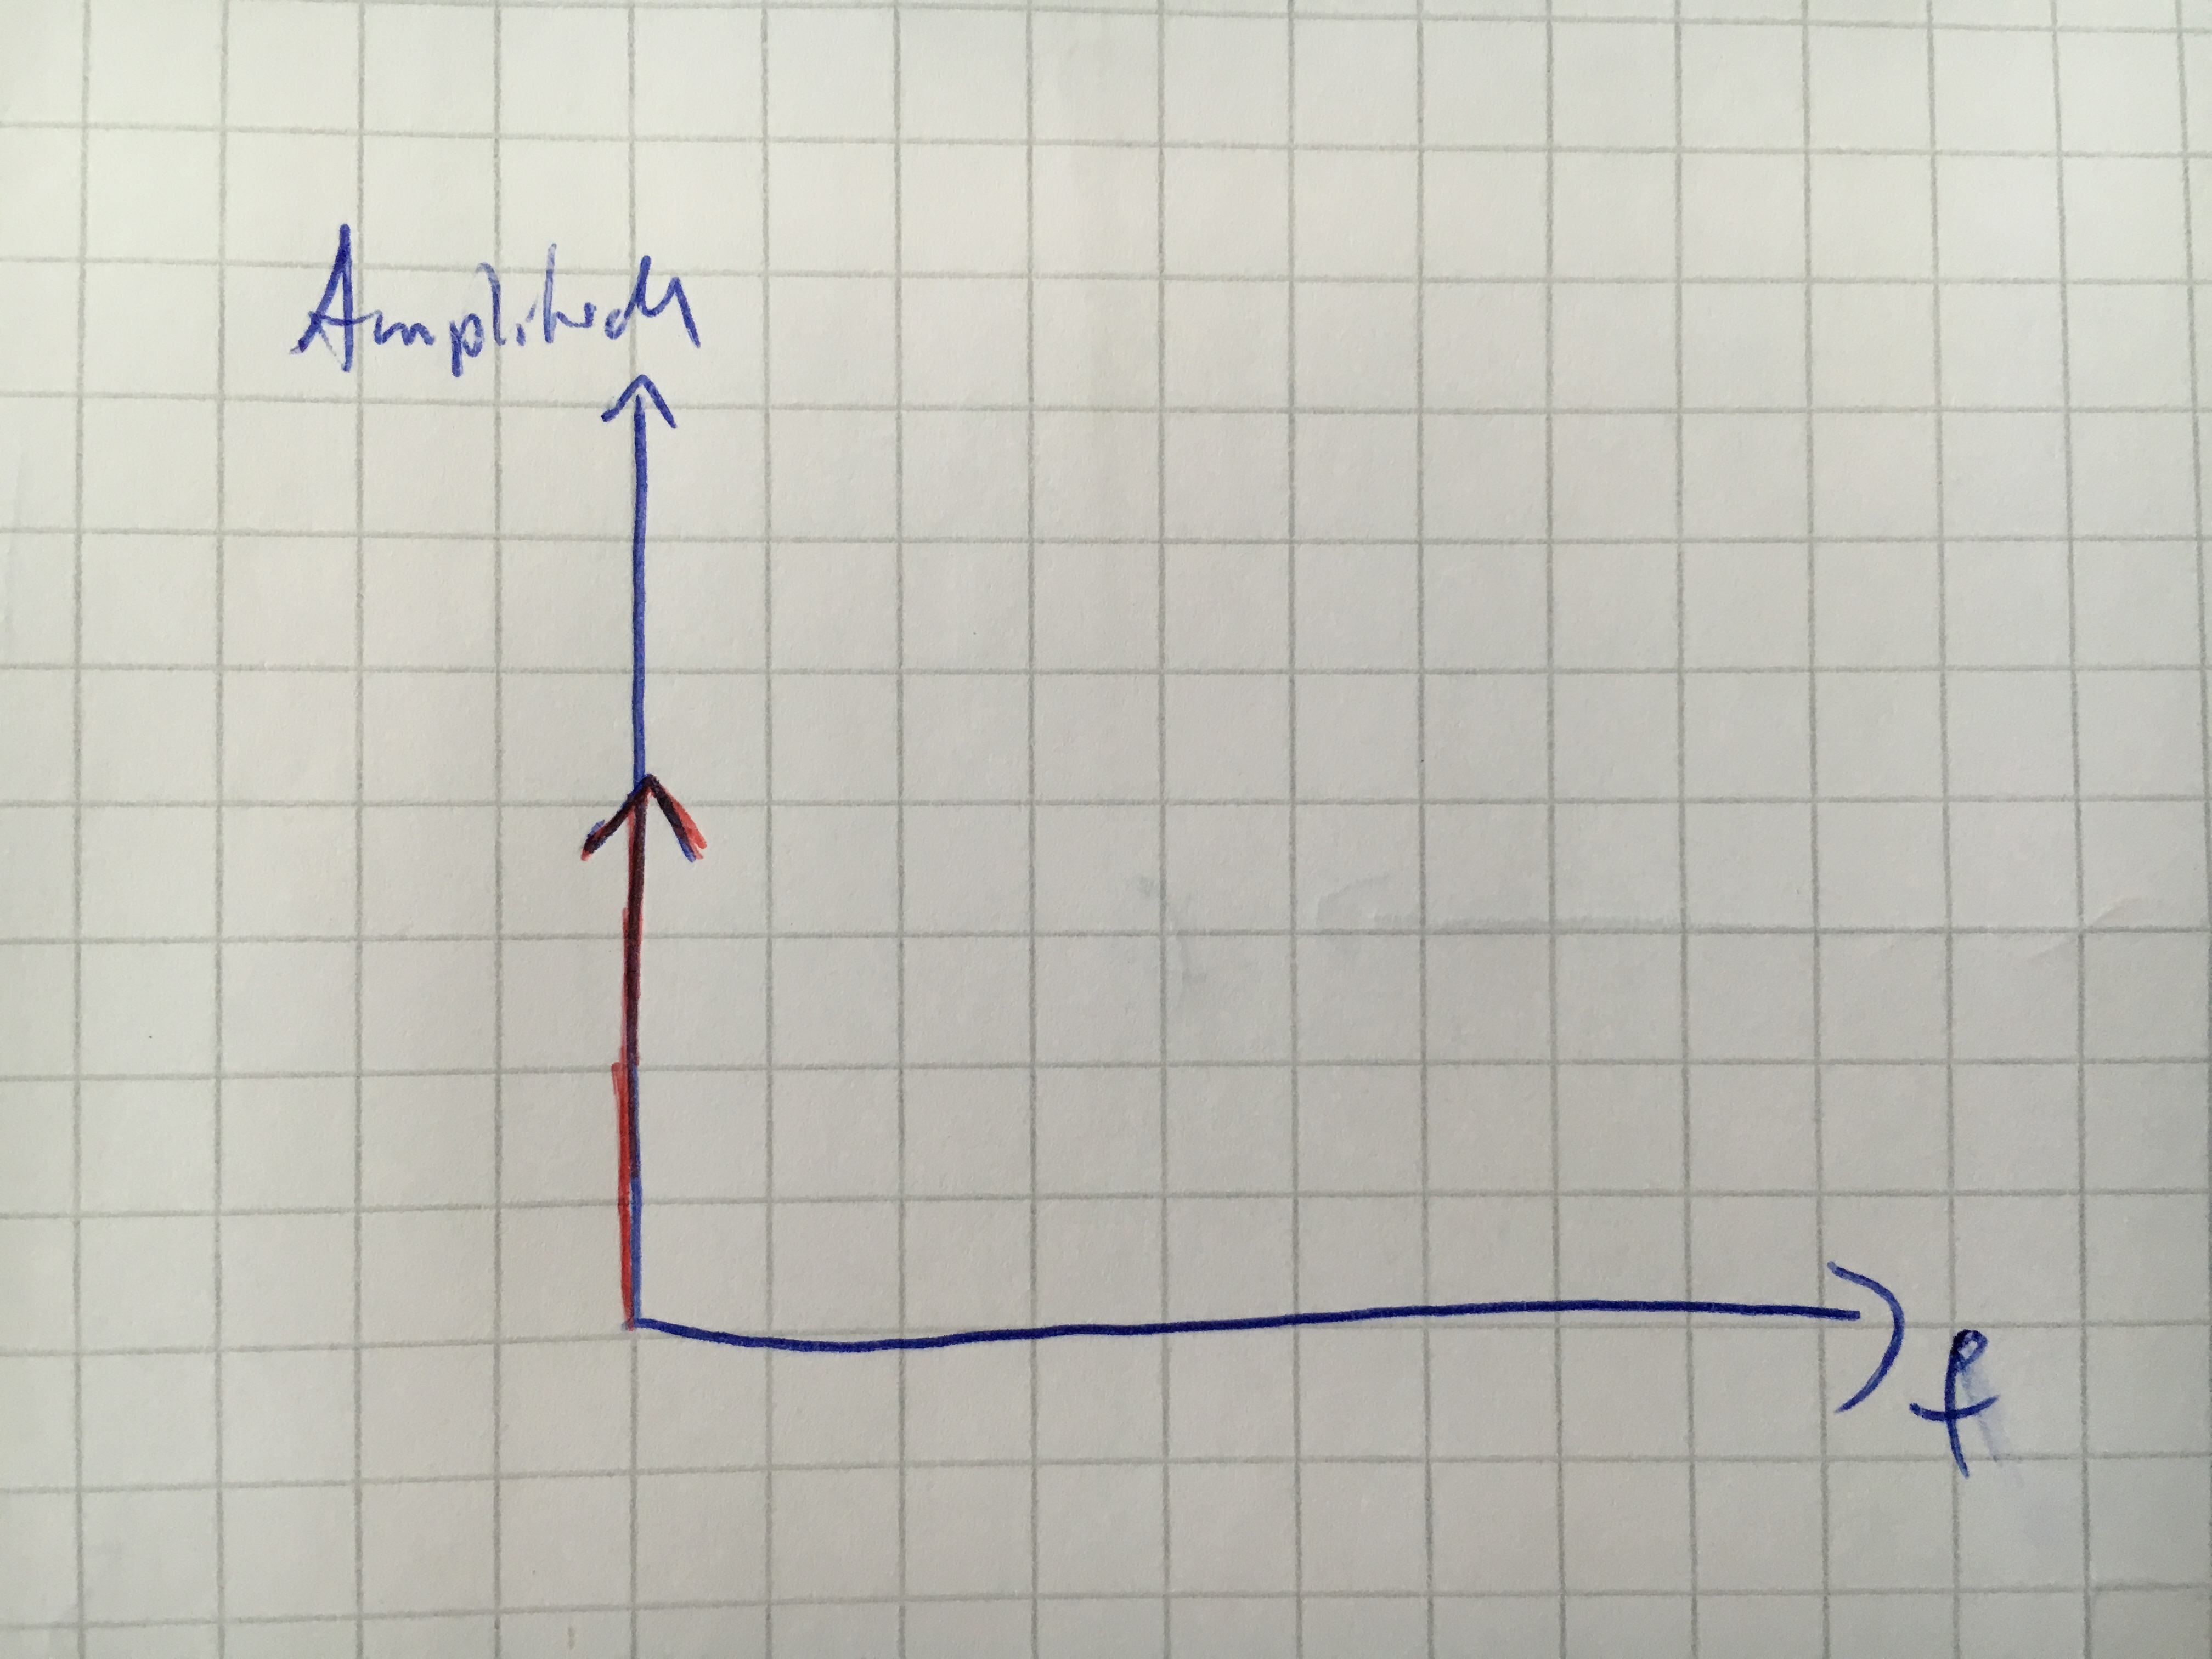
\includegraphics[width=\textwidth]{images/dc}
    \caption{DC Level function}
%    \label{fig:leakExplain}
  \end{minipage}
  \hfill
  \begin{minipage}[b]{0.45\textwidth}
    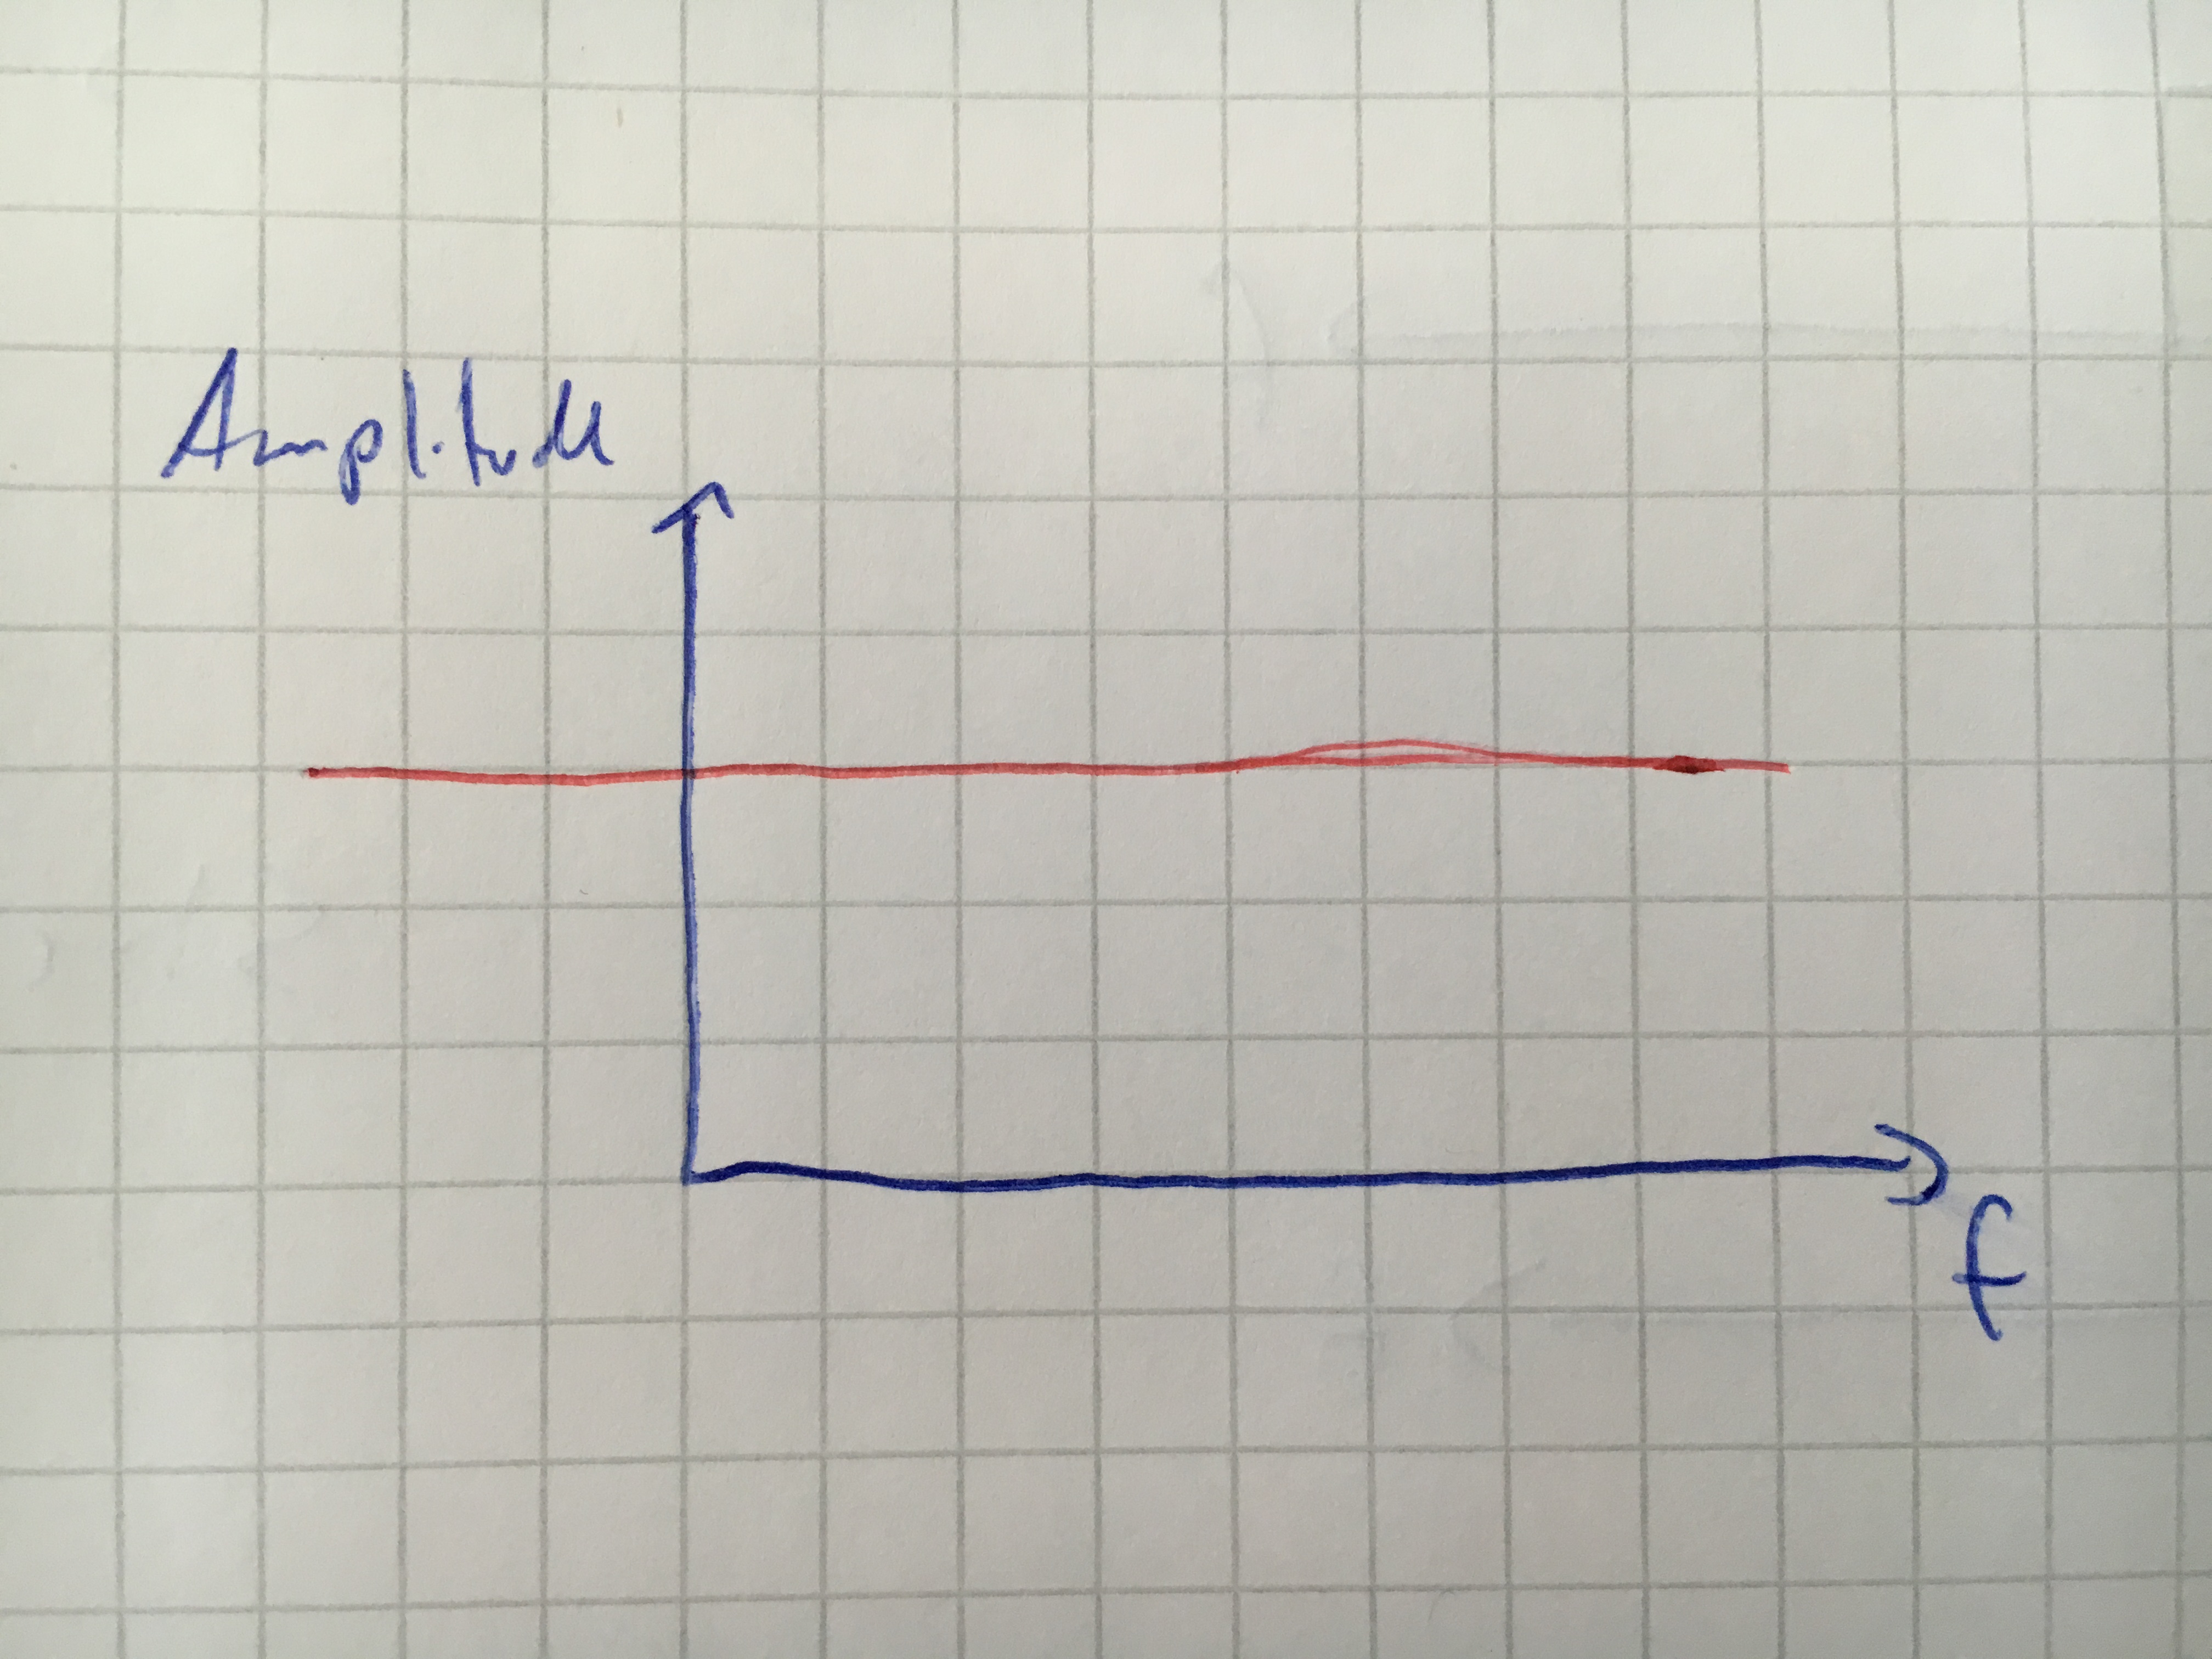
\includegraphics[width=\textwidth]{images/dirac}
    \caption{Dirac Function}
%    \label{fig:leak}
  \end{minipage}
\end{figure}

\begin{figure}[!htbp]
  \centering
  \begin{minipage}[b]{0.45\textwidth}
    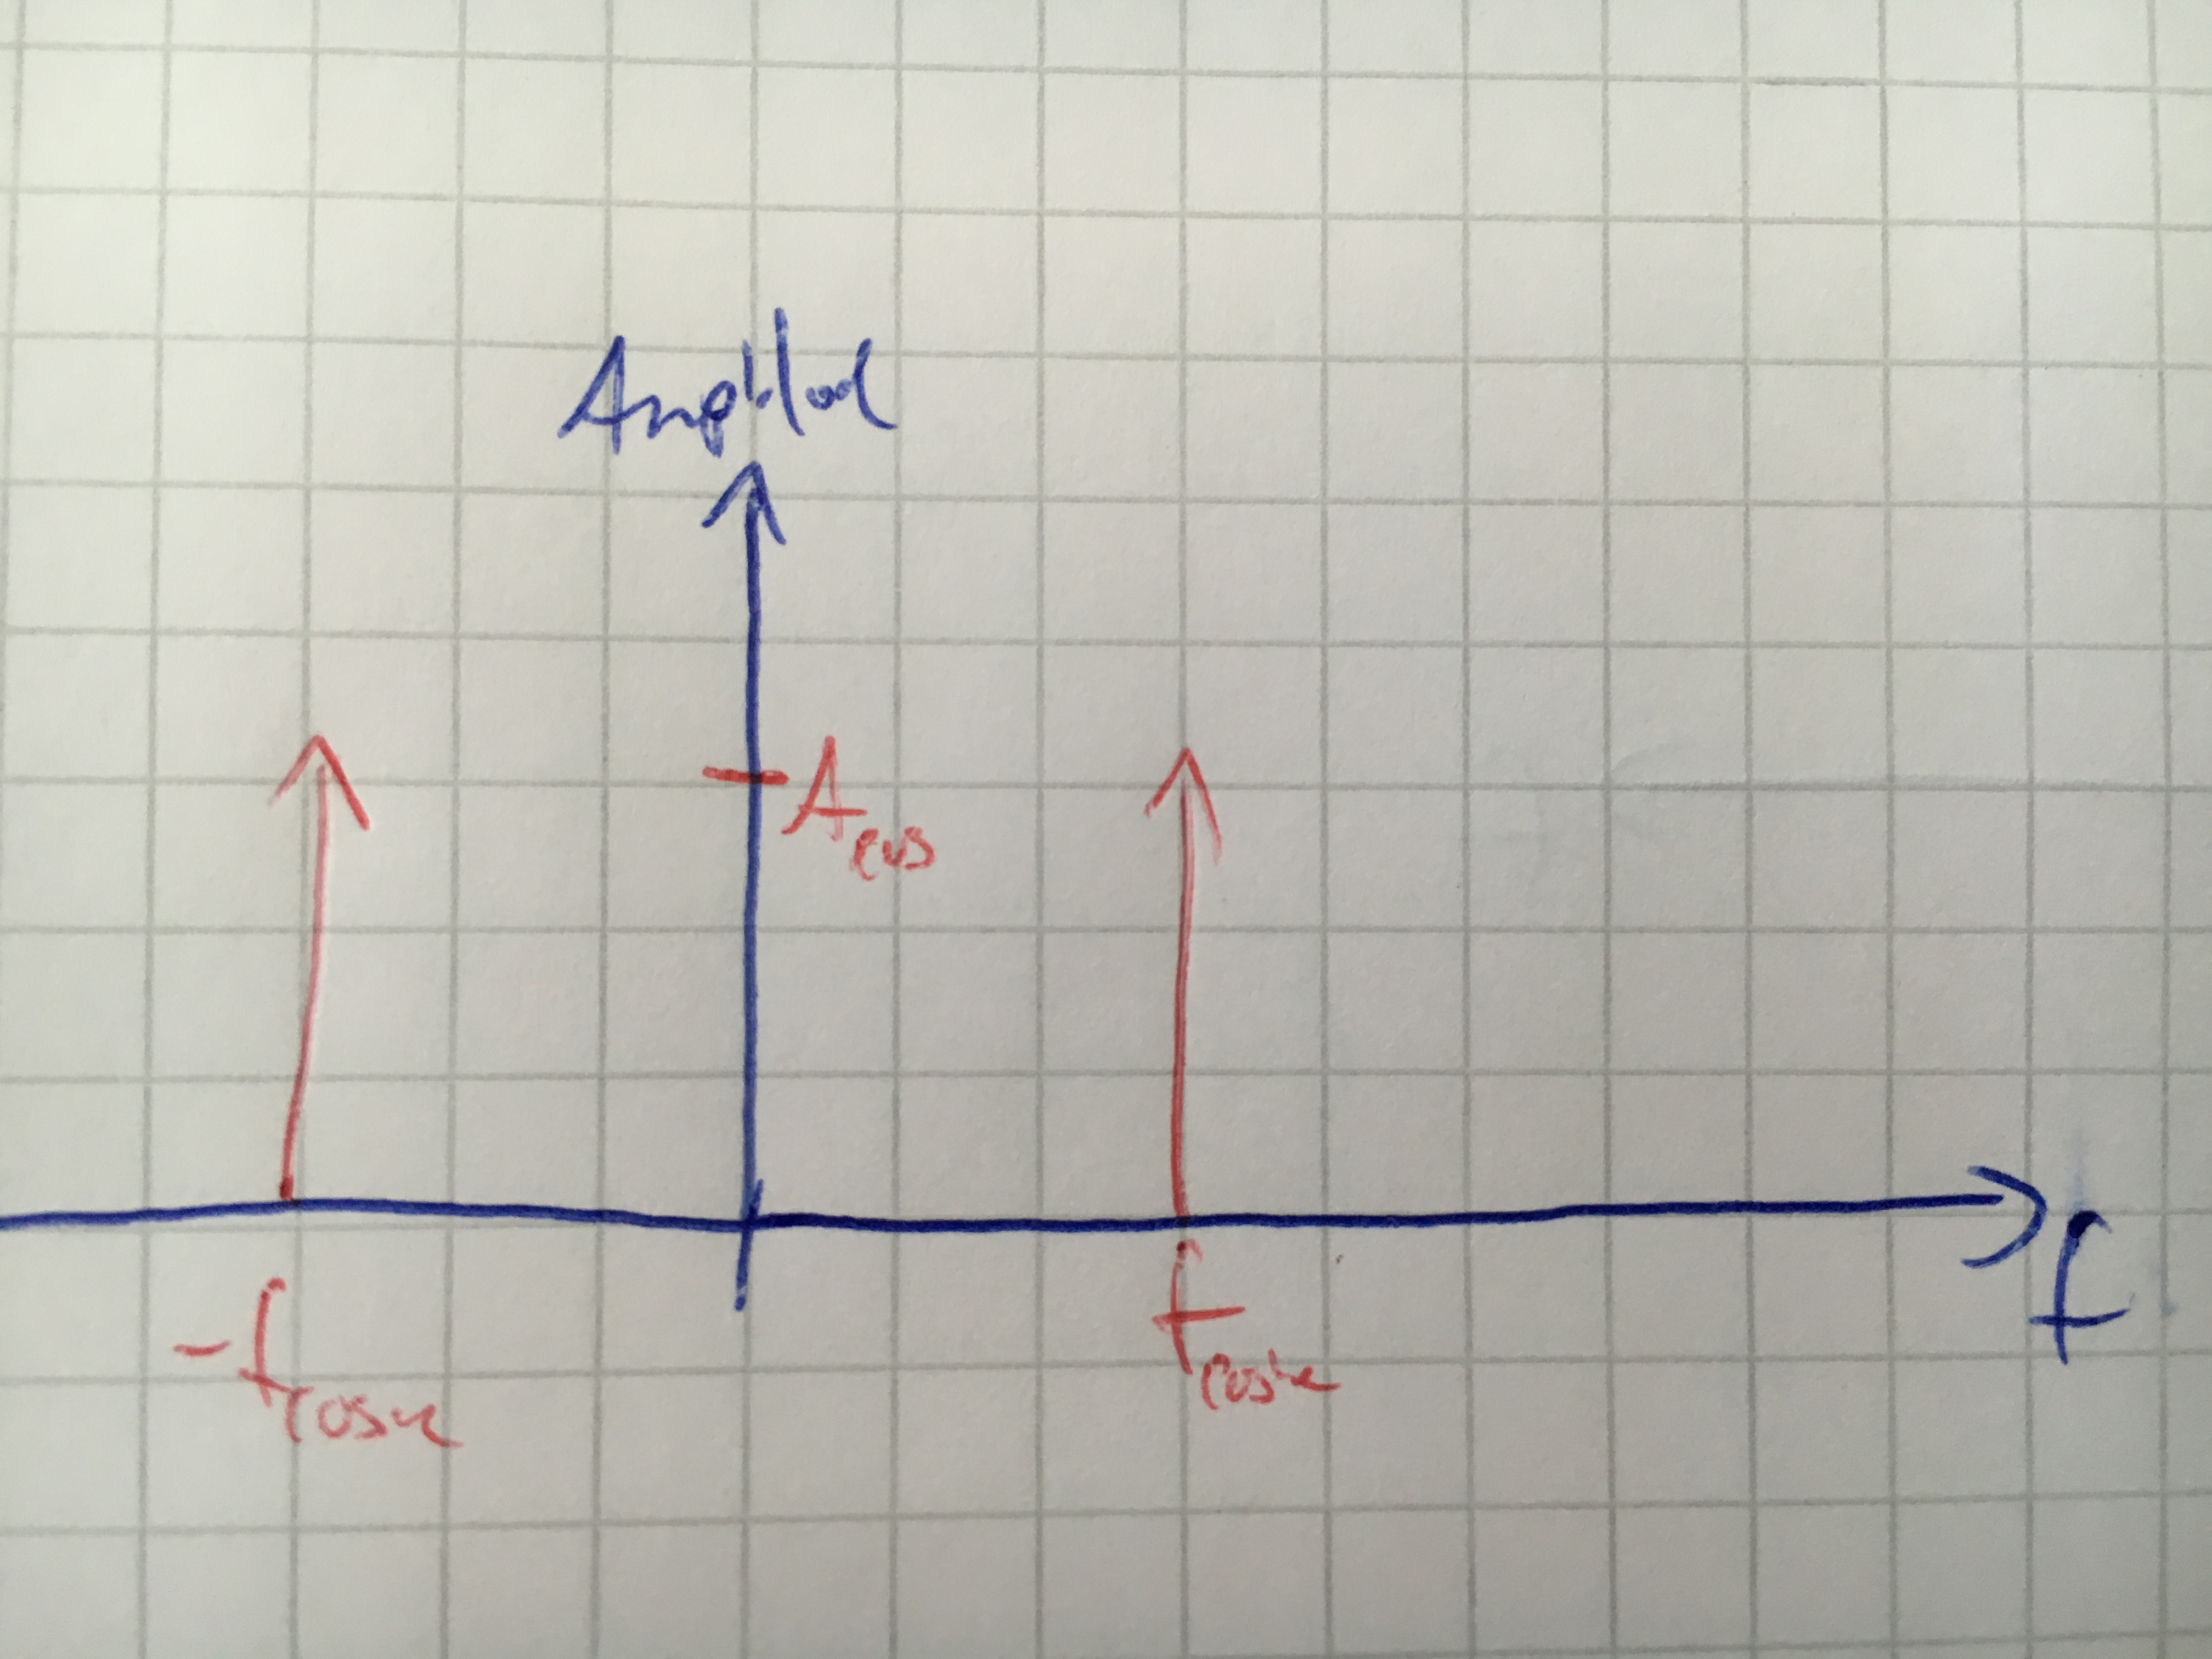
\includegraphics[width=\textwidth]{images/cosine}
    \caption{cosine with phase zero}
%    \label{fig:leakExplain}
  \end{minipage}
  \hfill
  \begin{minipage}[b]{0.45\textwidth}
    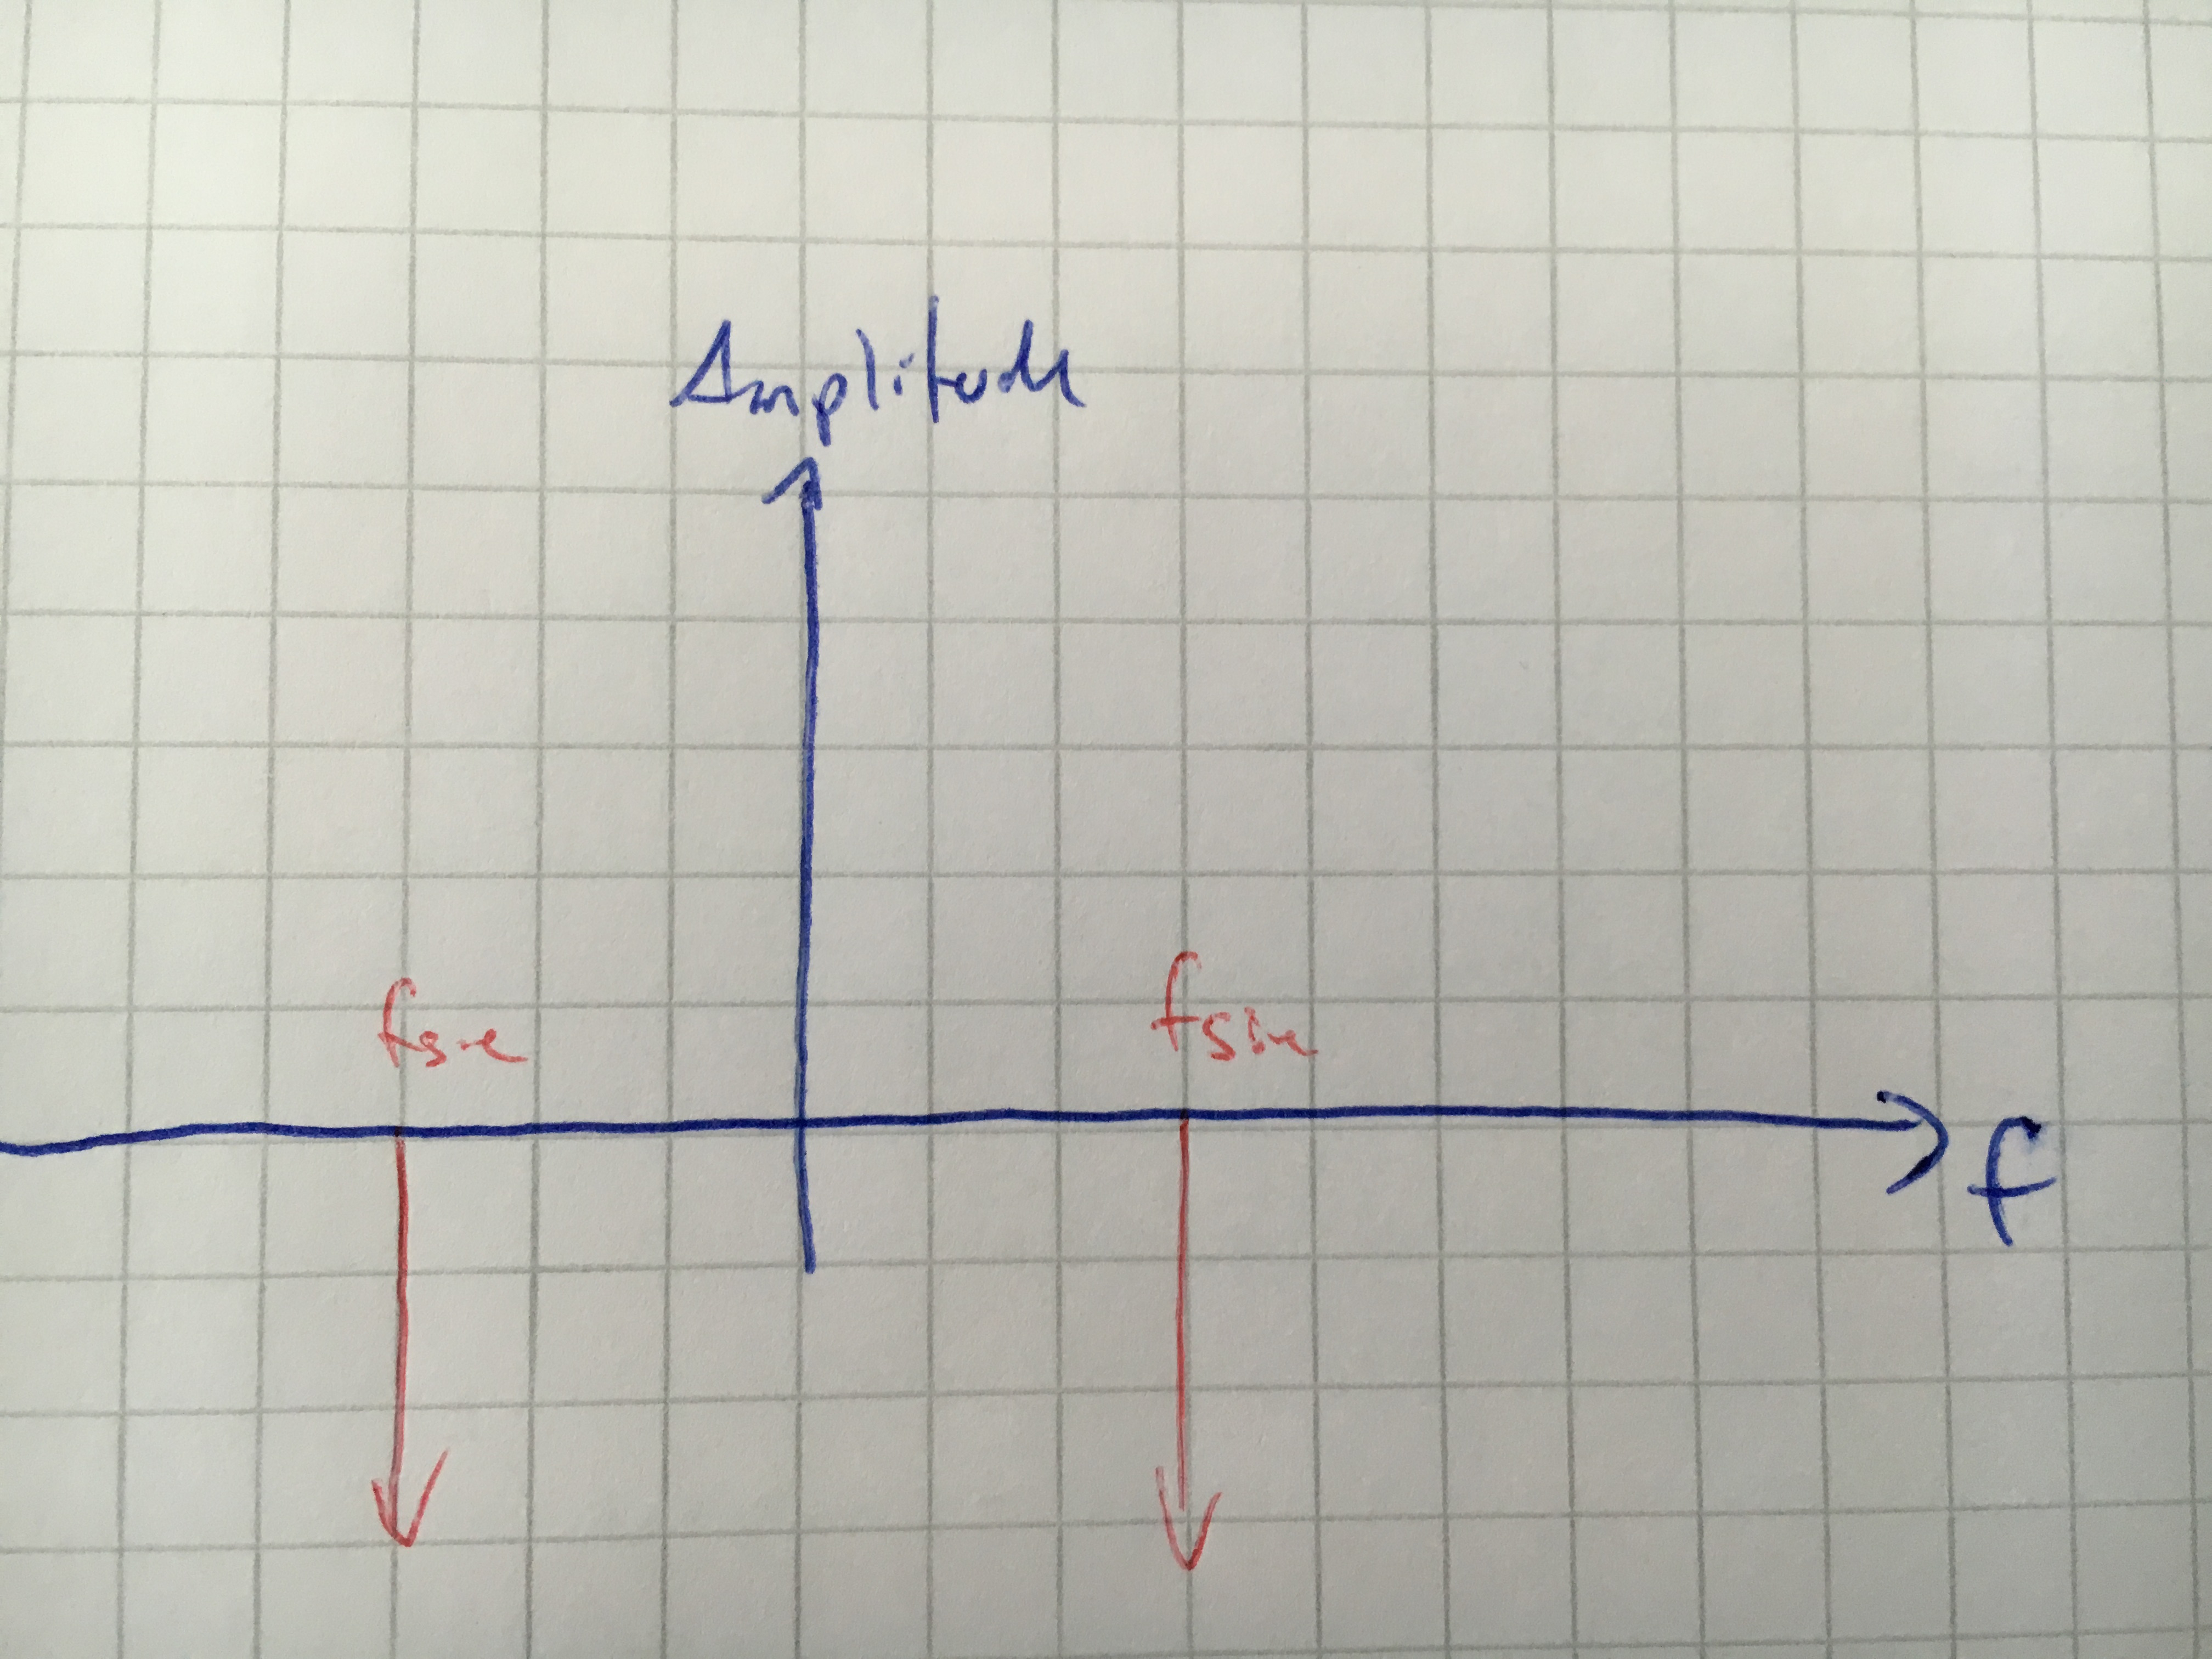
\includegraphics[width=\textwidth]{images/sine}
    \caption{sine with phase $\pi$/2}
%    \label{fig:leak}
  \end{minipage}
\end{figure}

\begin{figure}[!htbp]
  \centering
  \begin{minipage}[b]{0.45\textwidth}
    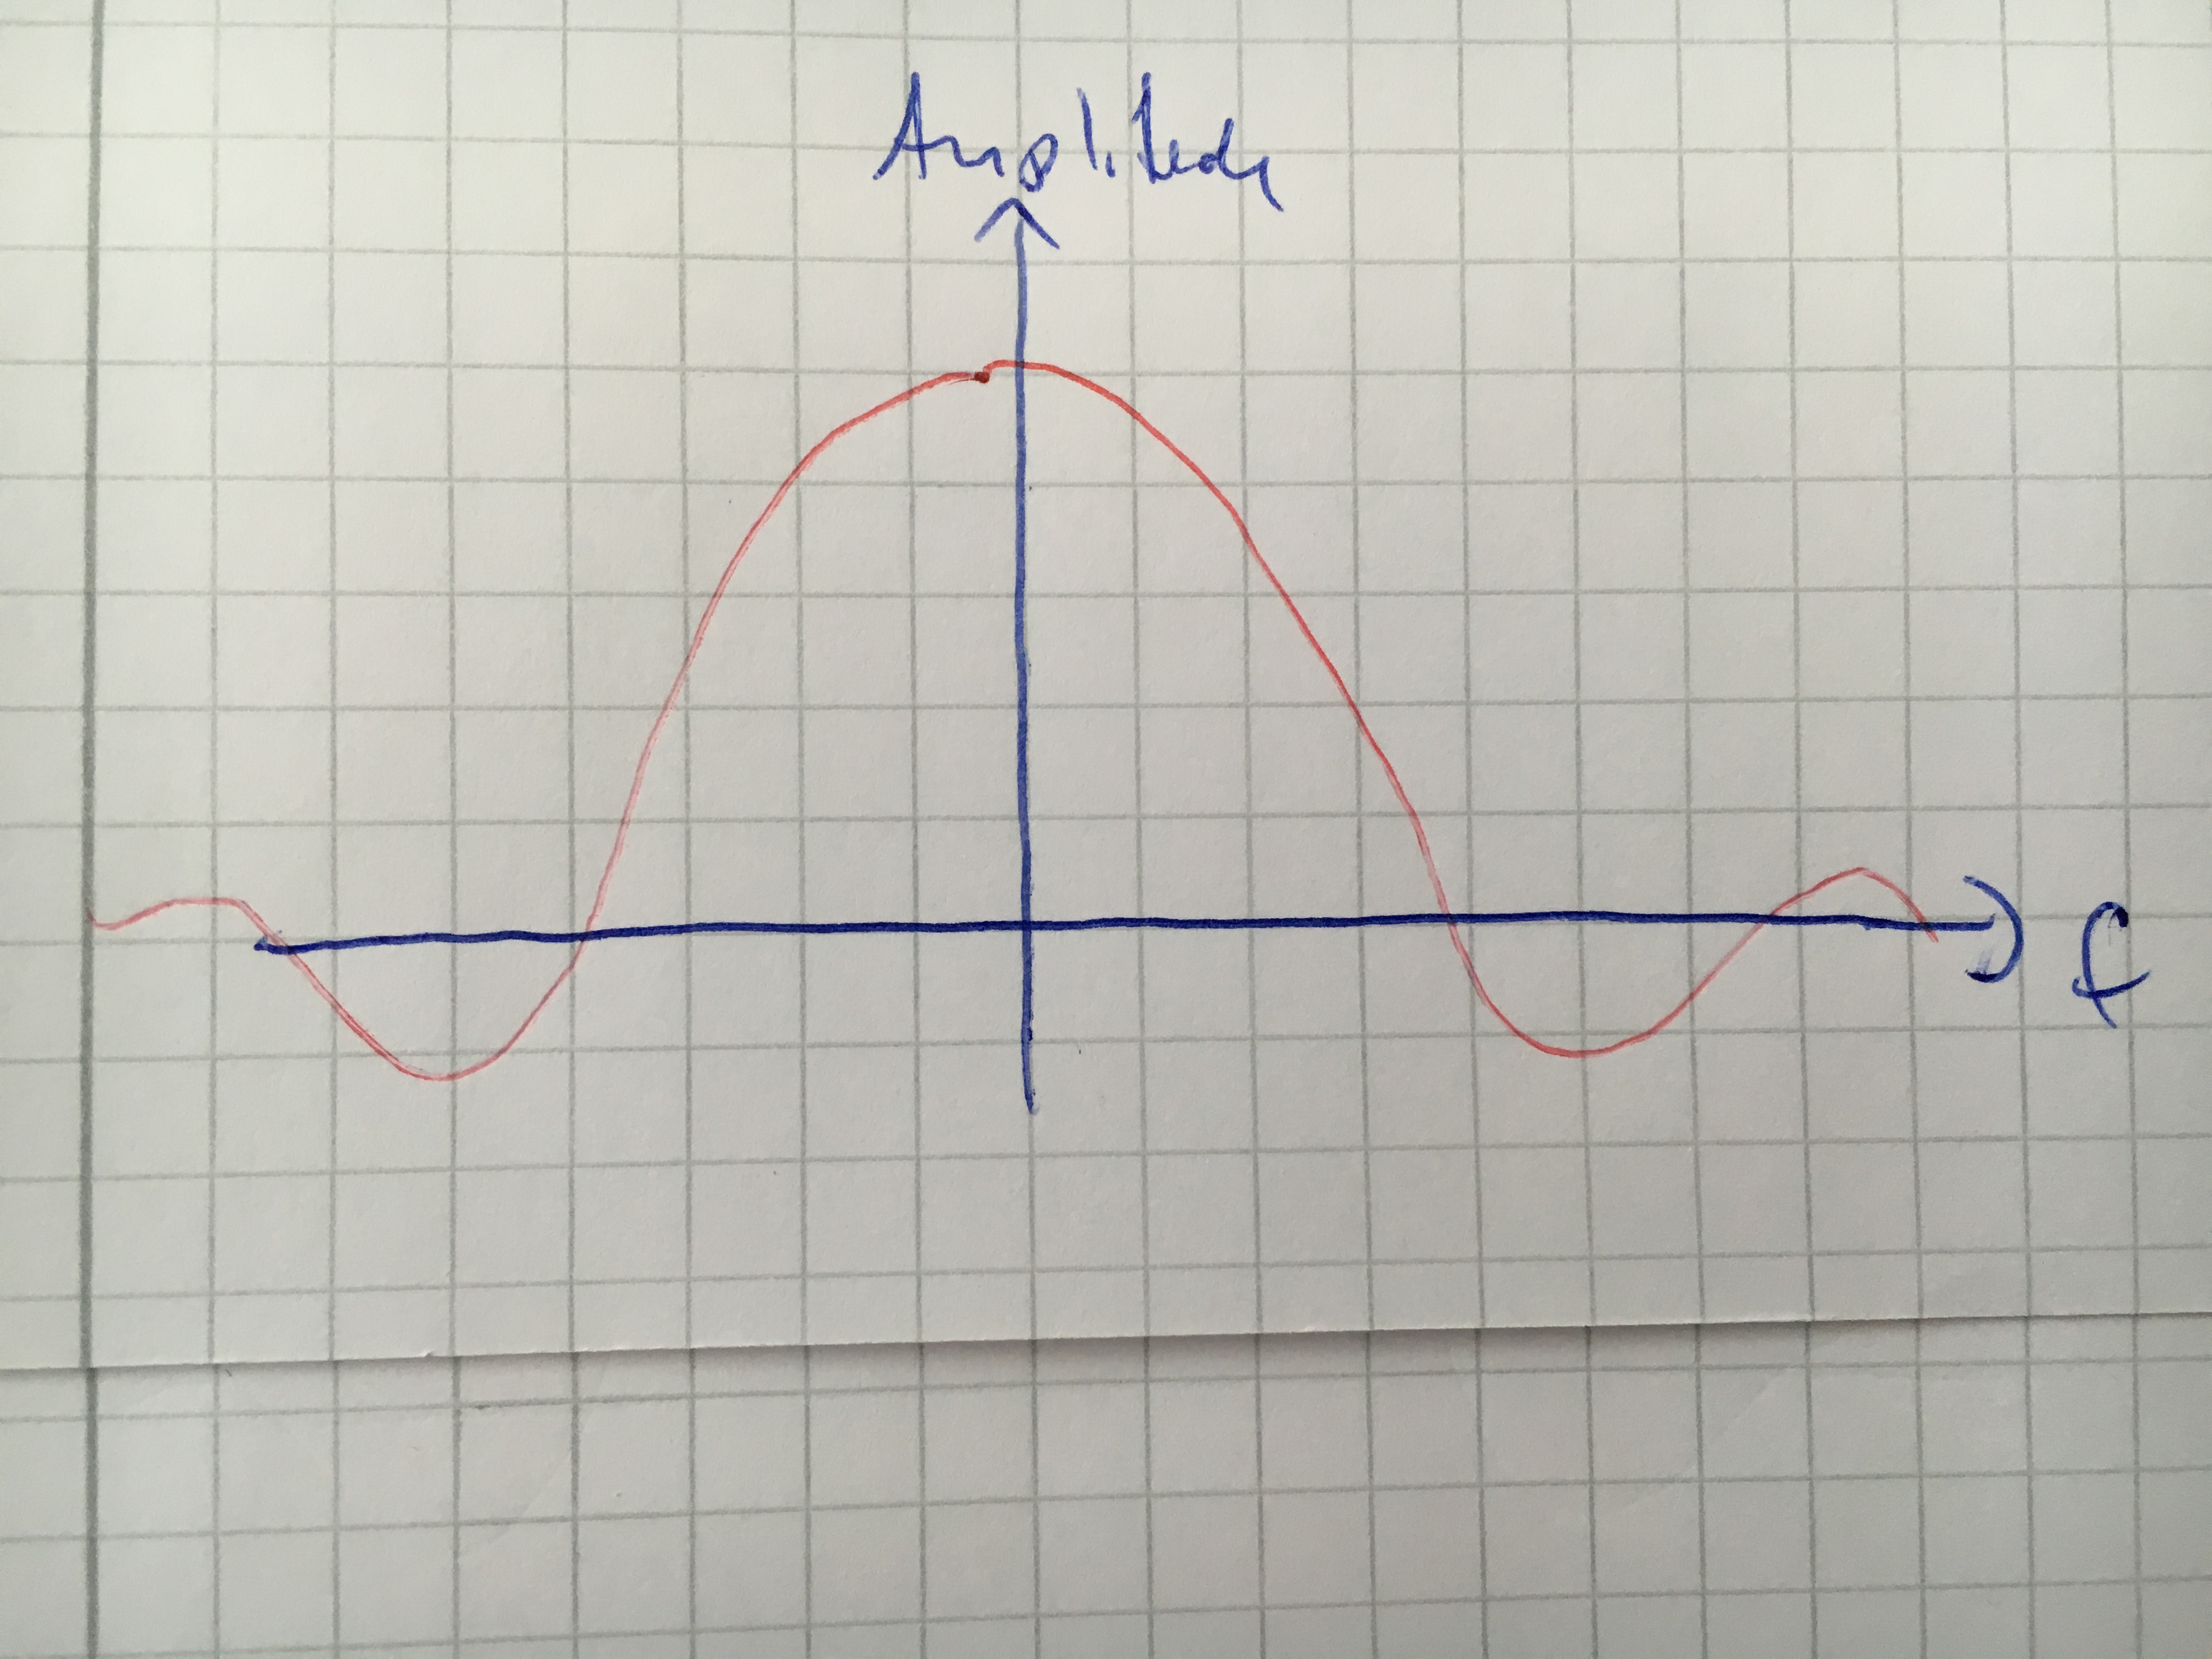
\includegraphics[width=\textwidth]{images/rect_narrow}
    \caption{Narrow rectangular function}
%    \label{fig:leakExplain}
  \end{minipage}
  \hfill
  \begin{minipage}[b]{0.45\textwidth}
    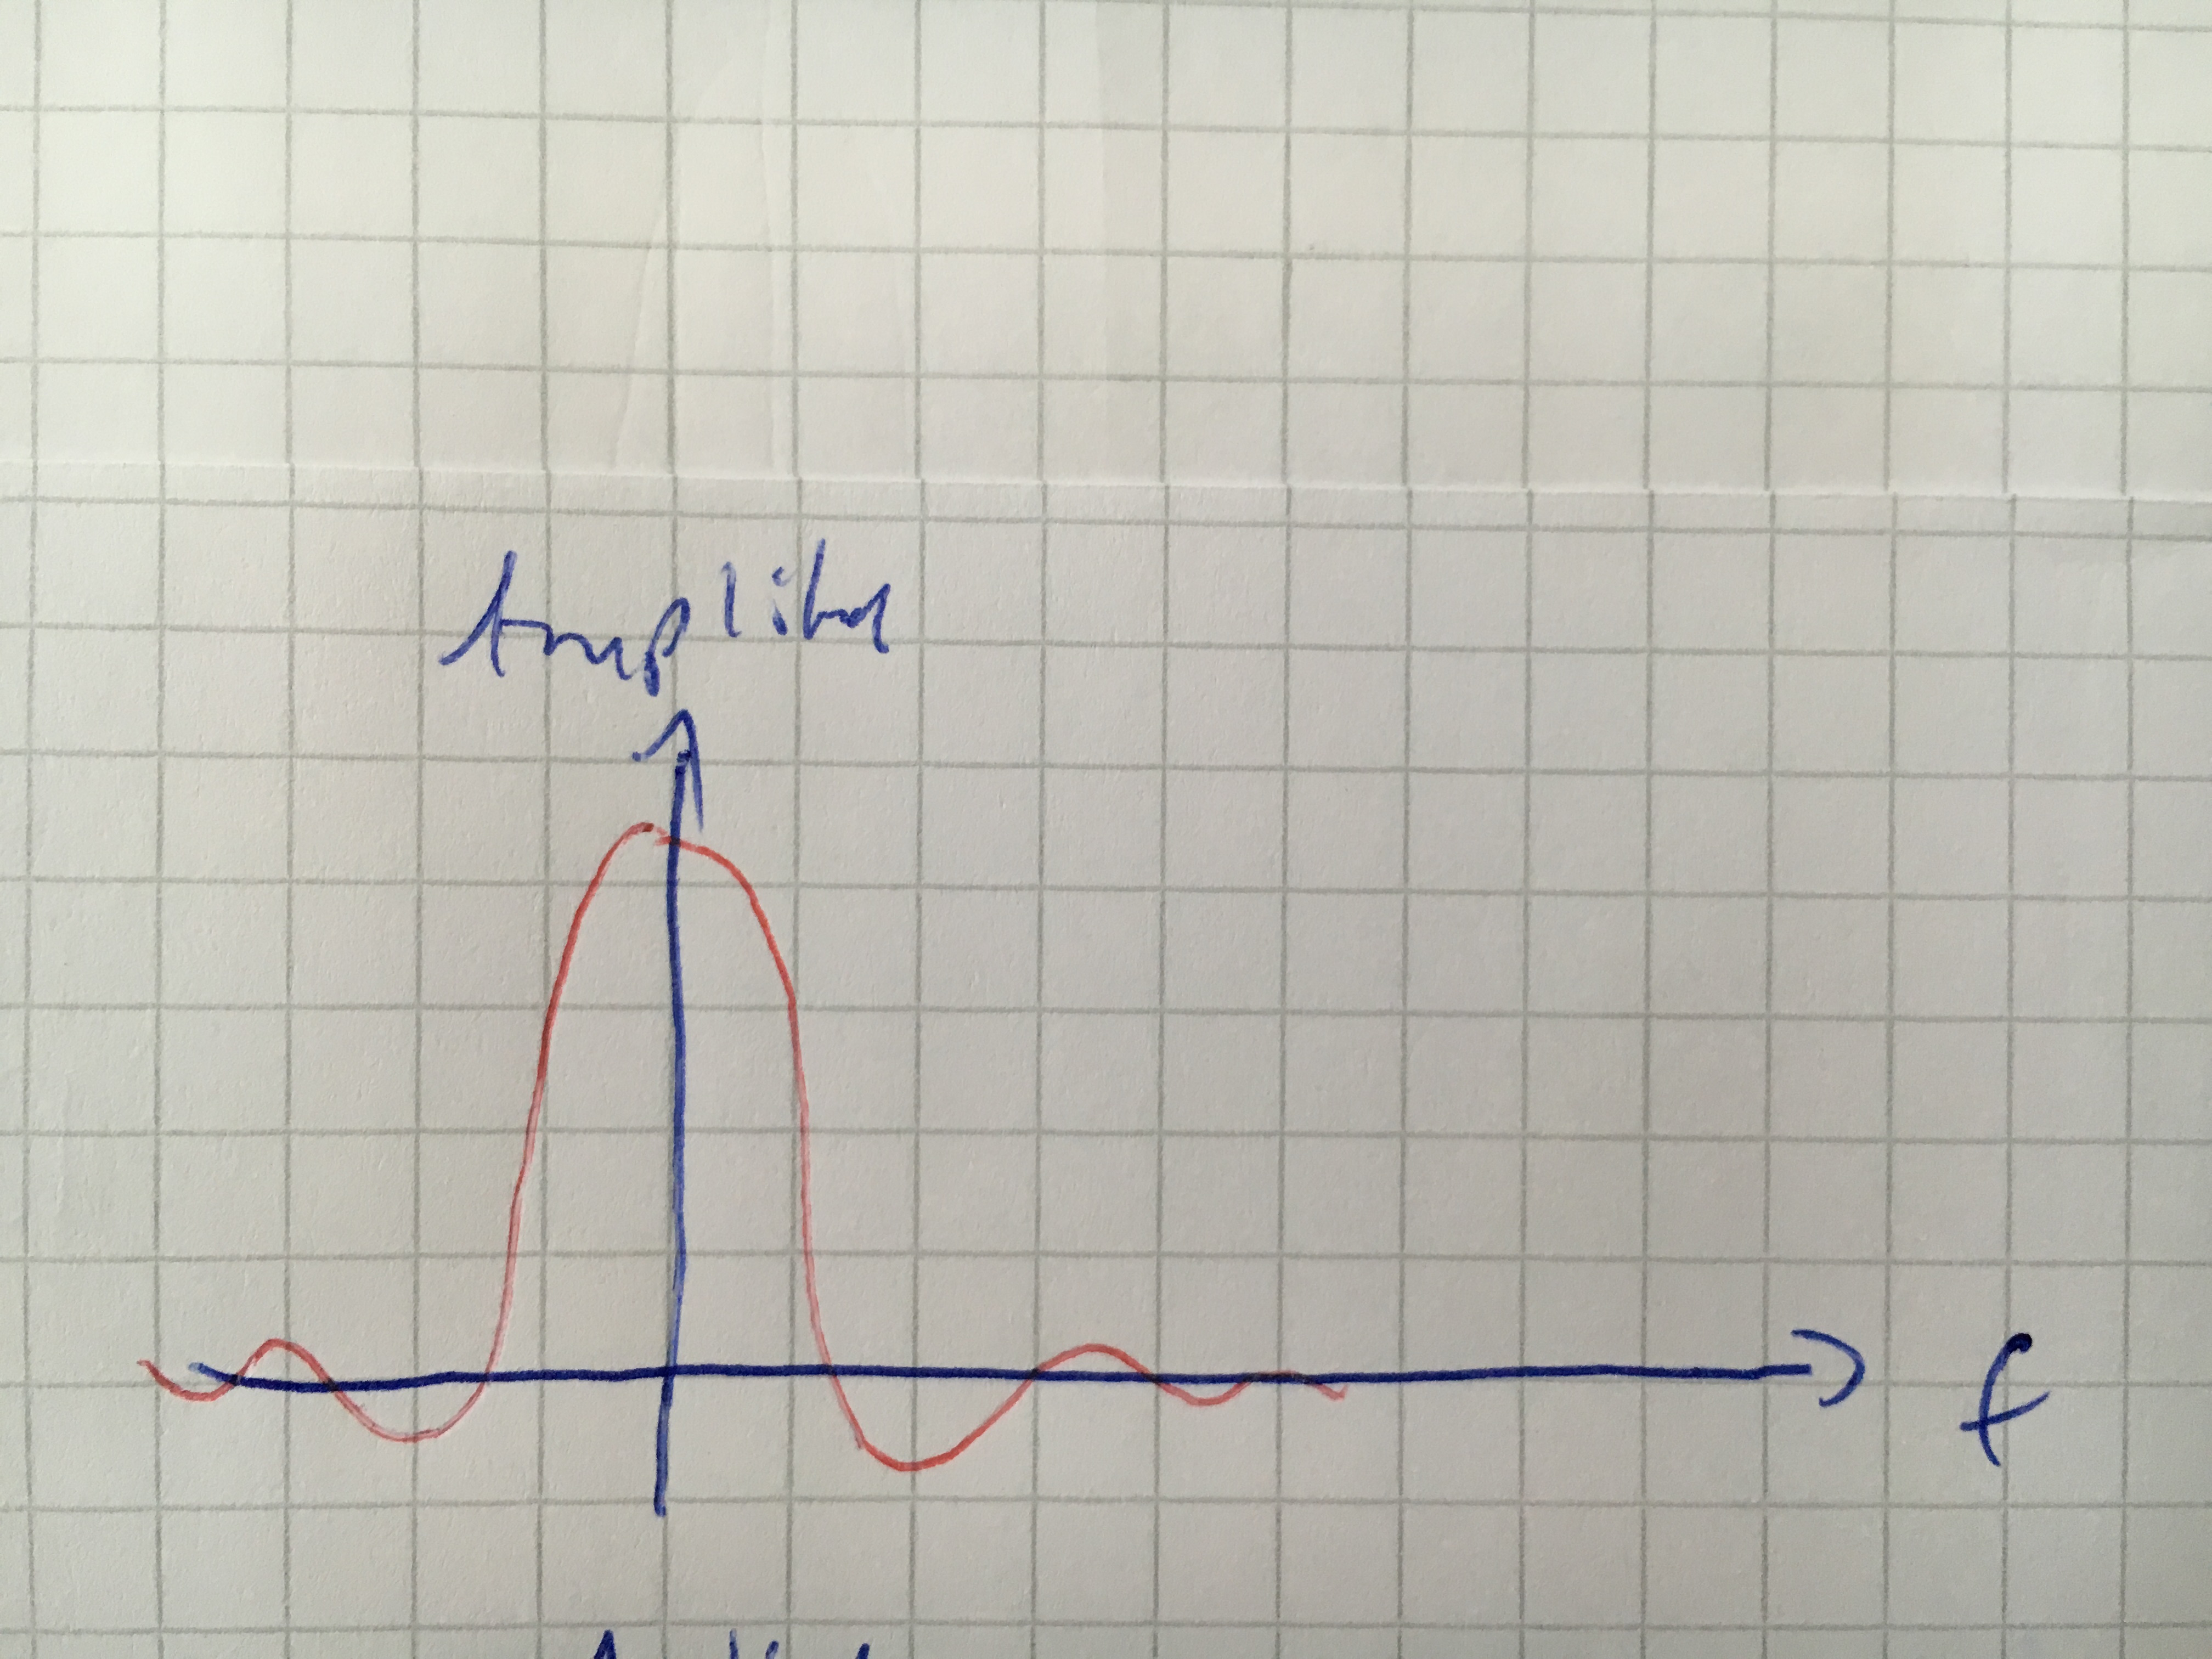
\includegraphics[width=\textwidth]{images/rect_broad}
    \caption{Broad rectangular function}
%    \label{fig:leak}
  \end{minipage}
\end{figure}


\begin{figure}[!htbp]
  \centering
  \begin{minipage}[b]{0.45\textwidth}
    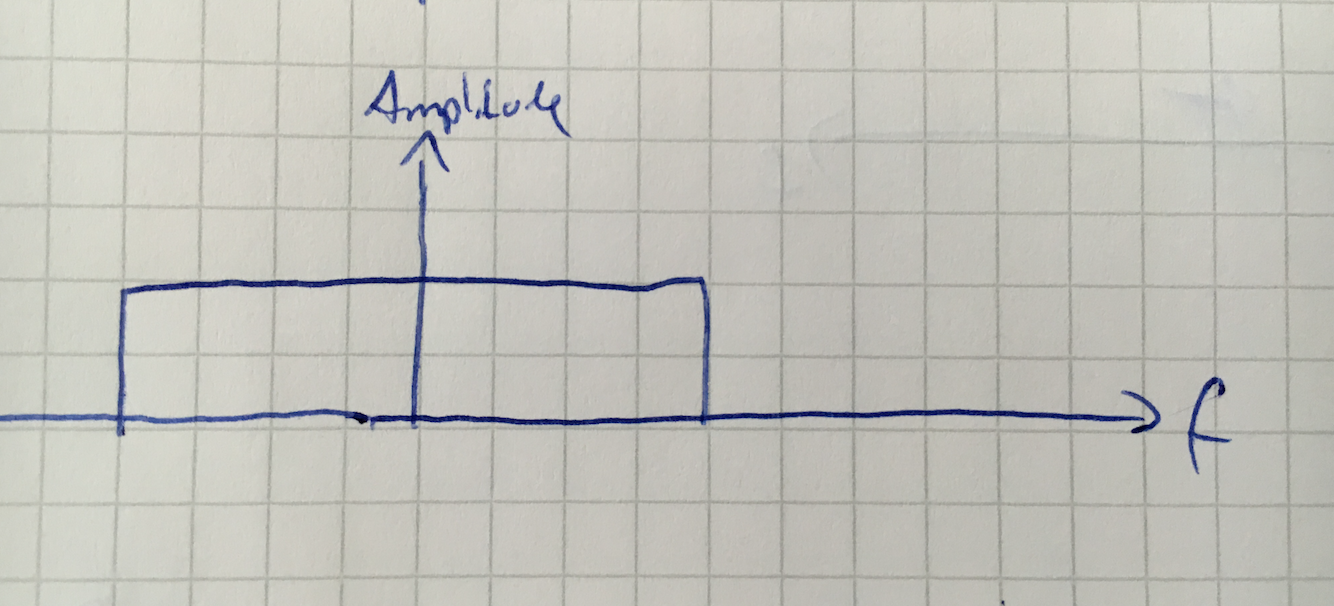
\includegraphics[width=\textwidth]{images/sinc_narrow}
    \caption{Narrow sinc function}
%    \label{fig:leakExplain}
  \end{minipage}
  \hfill
  \begin{minipage}[b]{0.45\textwidth}
    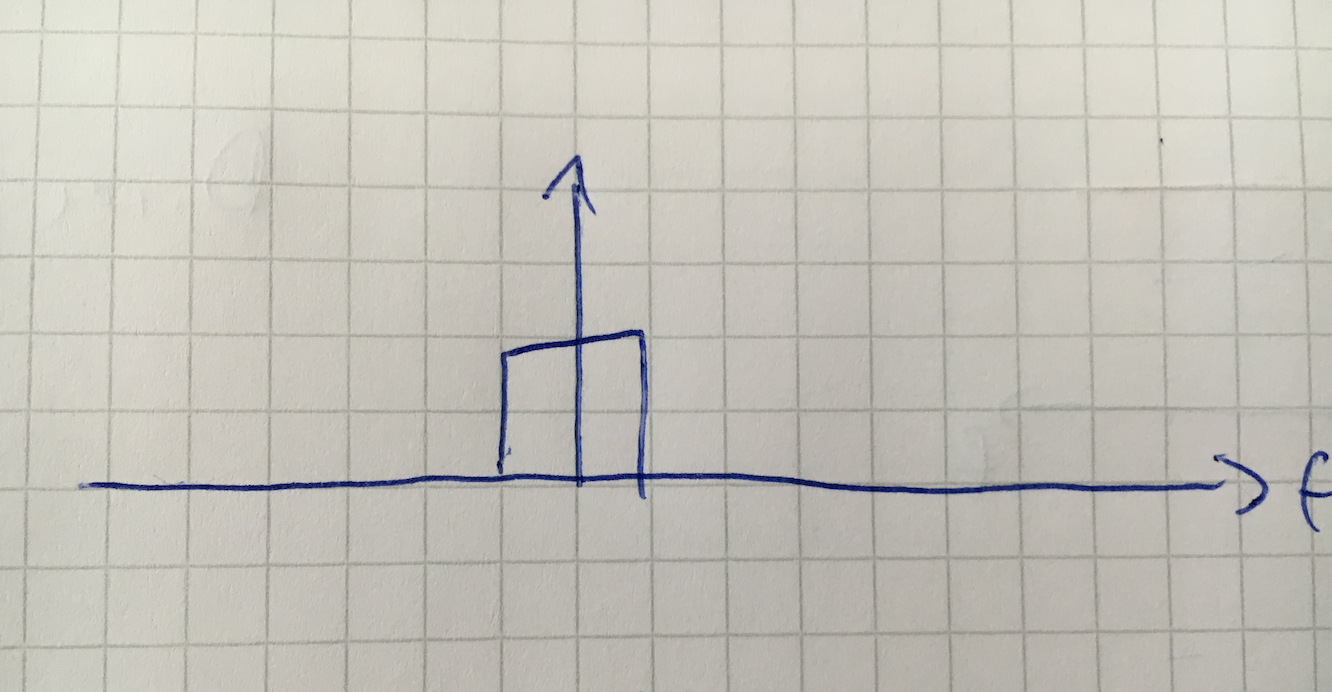
\includegraphics[width=\textwidth]{images/sinc_broad}
    \caption{Broad sinc function}
%    \label{fig:leak}
  \end{minipage}
\end{figure}

\begin{figure}[!htbp]
  \centering
  \begin{minipage}[b]{0.45\textwidth}
    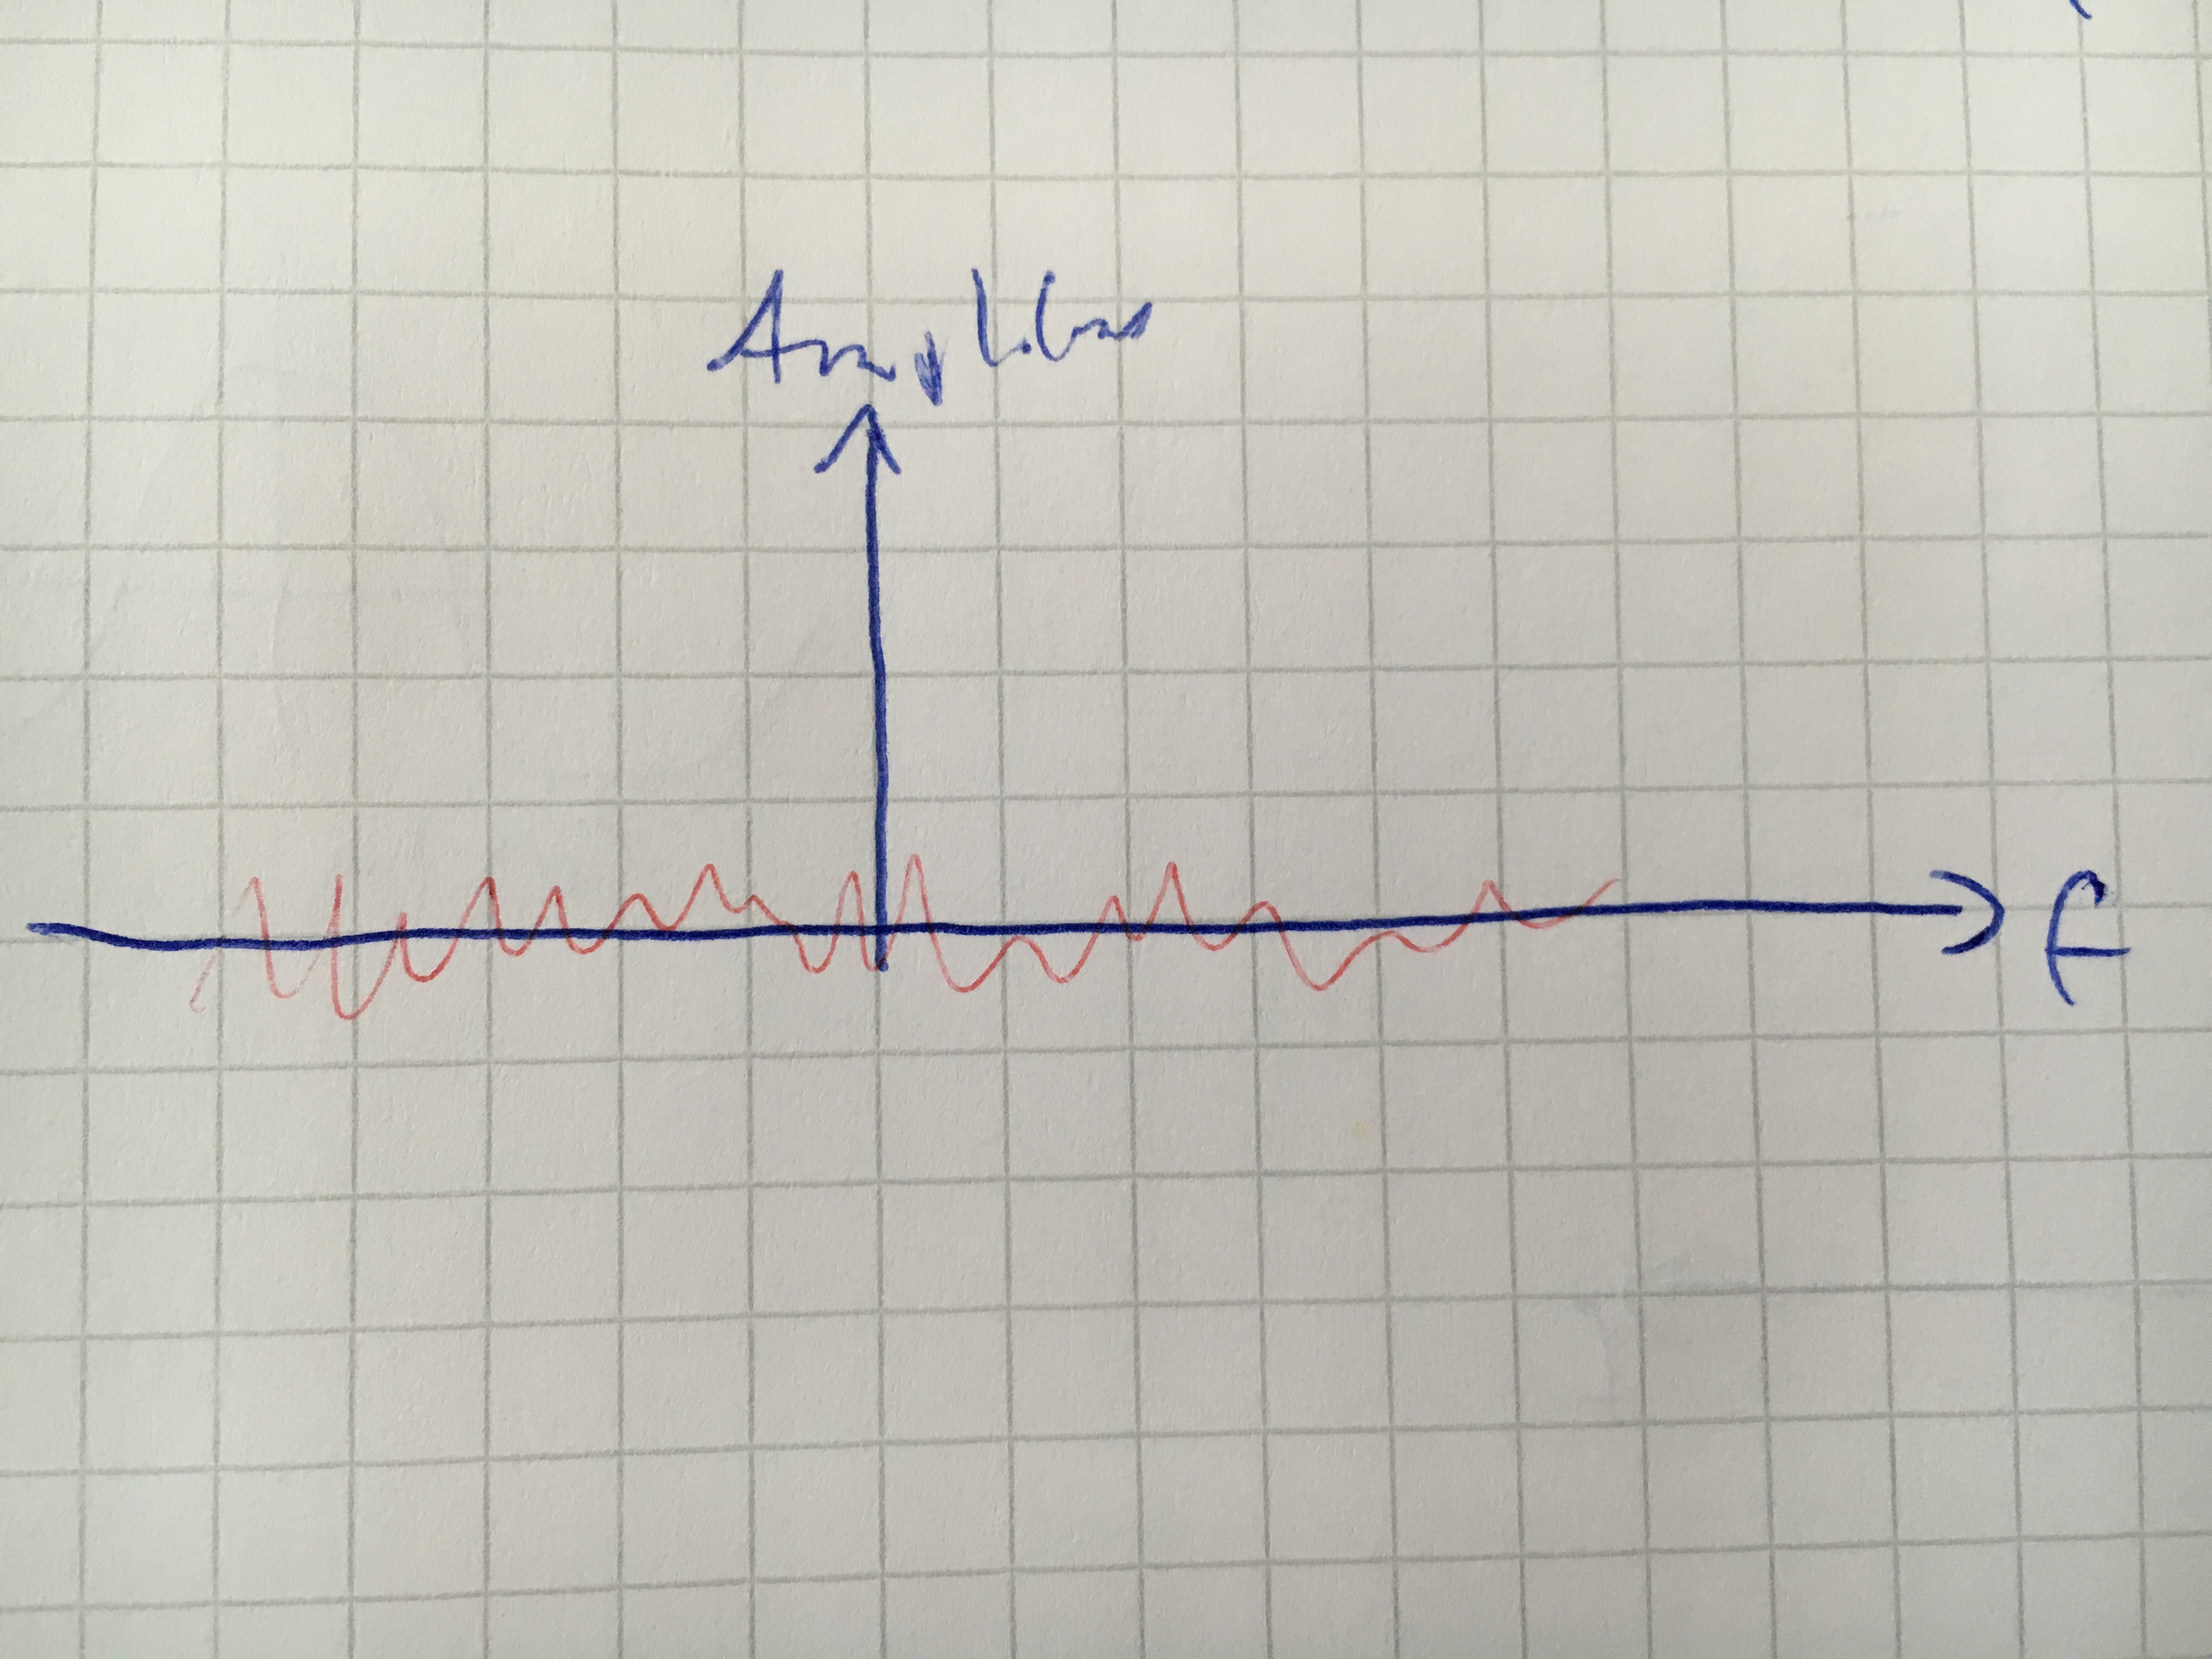
\includegraphics[width=\textwidth]{images/white}
    \caption{White Noise}
%    \label{fig:leakExplain}
  \end{minipage}
  \hfill
  \begin{minipage}[b]{0.45\textwidth}
%    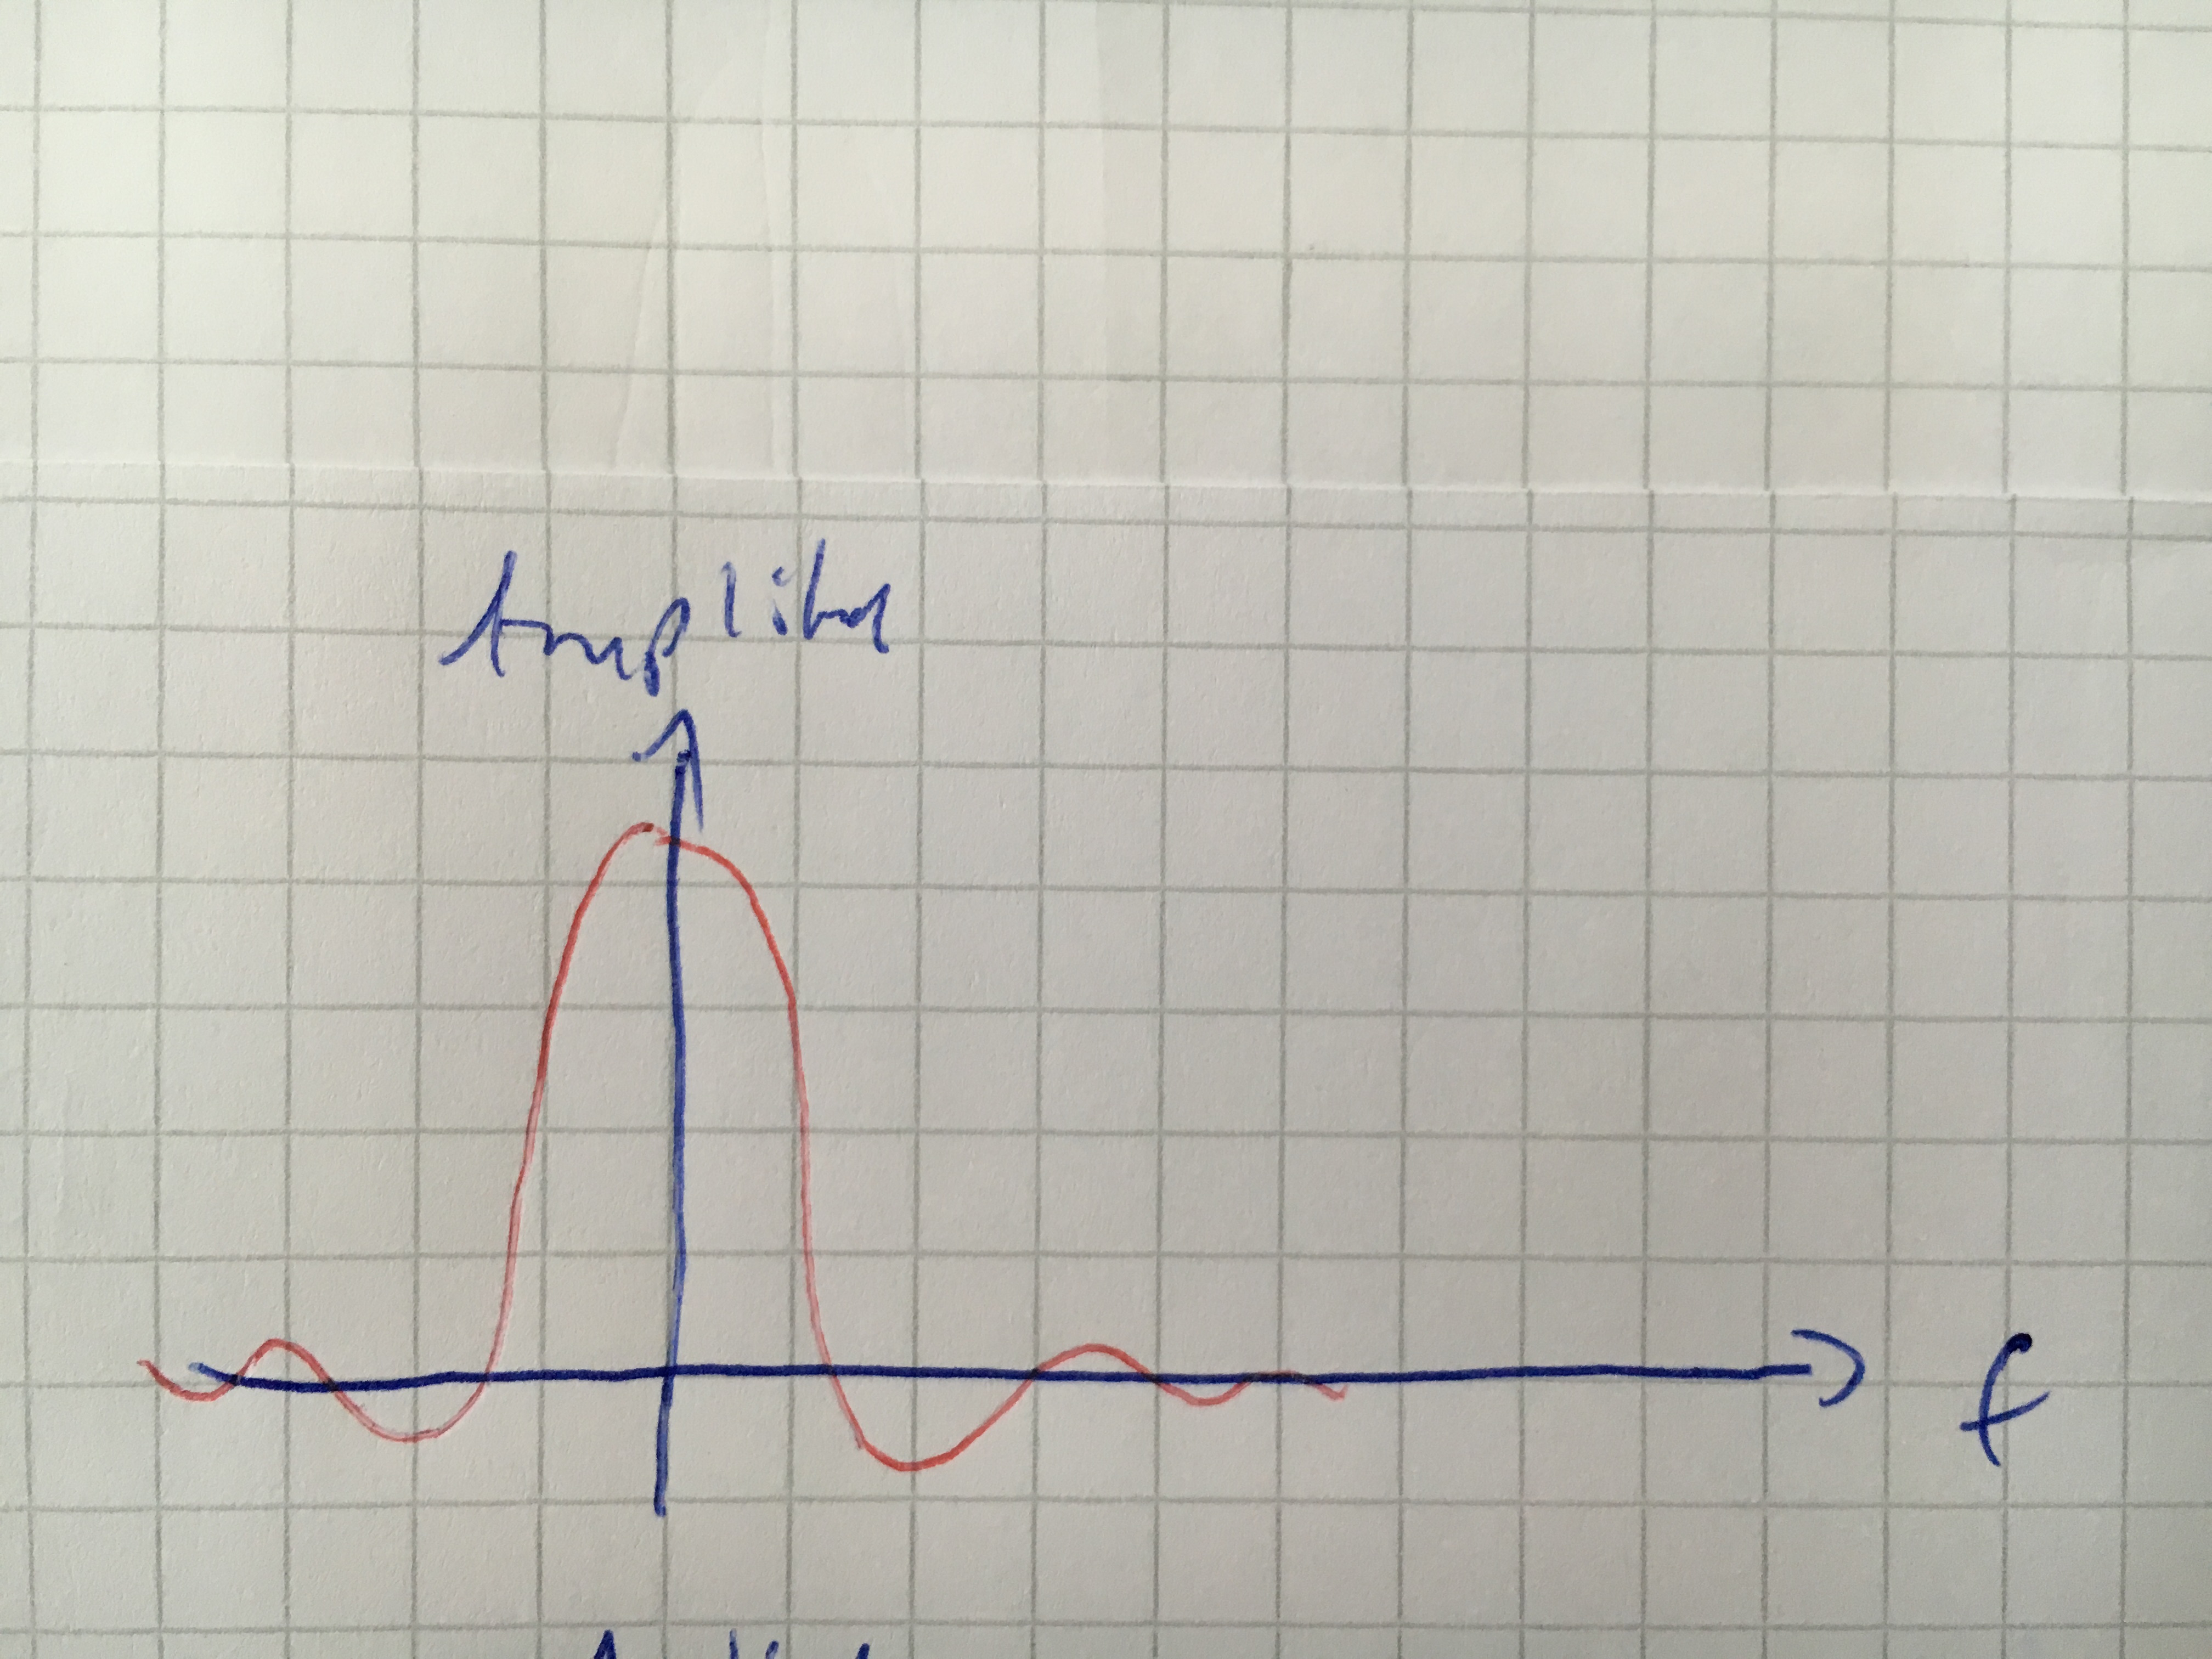
\includegraphics[width=\textwidth]{images/rect_broad}
%    \caption{Broad rectangular function}
%    \label{fig:leak}
  \end{minipage}
\end{figure}


\subsection{Discussion}
The spectrum of real valued, even functions has no imaginary part, whereas the spectrum of non-even function might have imaginary parts.

%%%%%%%%%%%%%%%%% TASK 2 %%%
\section{Sampling}
Three  harmonic functions, on the form x(t) = Acos($2 \pi ft + \varphi $) are plotted in figure \ref{fig:sampling}.

\begin{figure}[h]
	\centering
	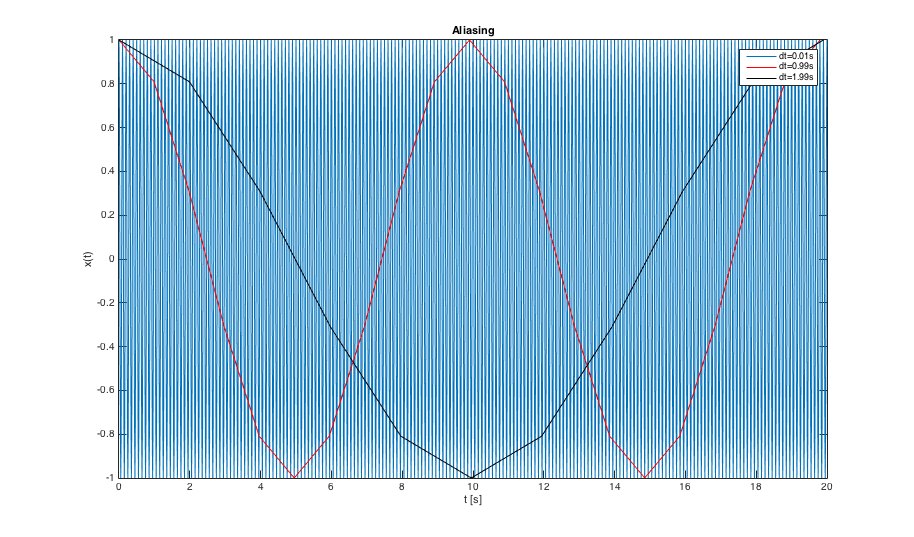
\includegraphics[width=\linewidth]{images/ass1_2}	
	\caption{Aliased harmonic functions}
	\label{fig:sampling}
\end{figure}
The two Aliasing frequencies are determined by reading the time period for one period of the respective harmonic function.
The two Aliasing frequencies are:

\begin{itemize}
	\item 0.1 Hz (red line)
	\item 0.05 Hz (blue line)
\end{itemize}

An appropriate expression for the aliasing frequency is given as follows:
\begin{equation}
\centering
	f_{alias}(N) = f - N f_{S}
	\label{eq:alias}
\end{equation}

where $f$ is the signal frequency and $N$ represents an appropriate integer value.


%%%%%%%%%%%%%%%%% TASK 3 %%%
%\section{DFT}
\addtocounter{section}{1}


%%%%%%%%%%%%%%%%% TASK 4 %%%
\section{Amplitude Diagram}
Power of Sum is like summing the power of each
In Figure \ref{fig:amplitude} the DFT of three harmonic functions with different amplitudes is shown. In MATLAB the \textit{fft}-function\footnote{Fast Fourier Transform} was used.
\begin{figure}[h!]
	\centering
	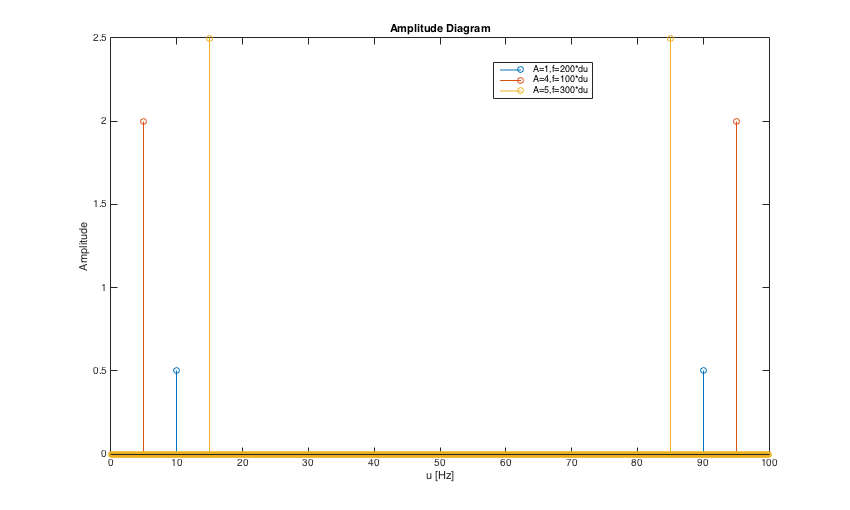
\includegraphics[width=\linewidth]{images/ass1_4}	
	\caption{Three functions with different Amplitudes}
	\label{fig:amplitude}
\end{figure}

As one can see, it does not matter in which order the requested operation, the power of the sum of two functions, is processed. The power of the sum of two functions is the same as the sum of the power of two functions, in the DFT.
Whereas the power of the signal is the squared magnitude of the frequency (\textit{note:} The x axis in the plot is shifted to the left. An appropriate double side diagram would have the origin point at, in this case, 50u).


%%%%%%%%%%%%%%%%% TASK 5 %%%
\section{Leakage}

%\begin{figure}[h!]
%	\centering
%	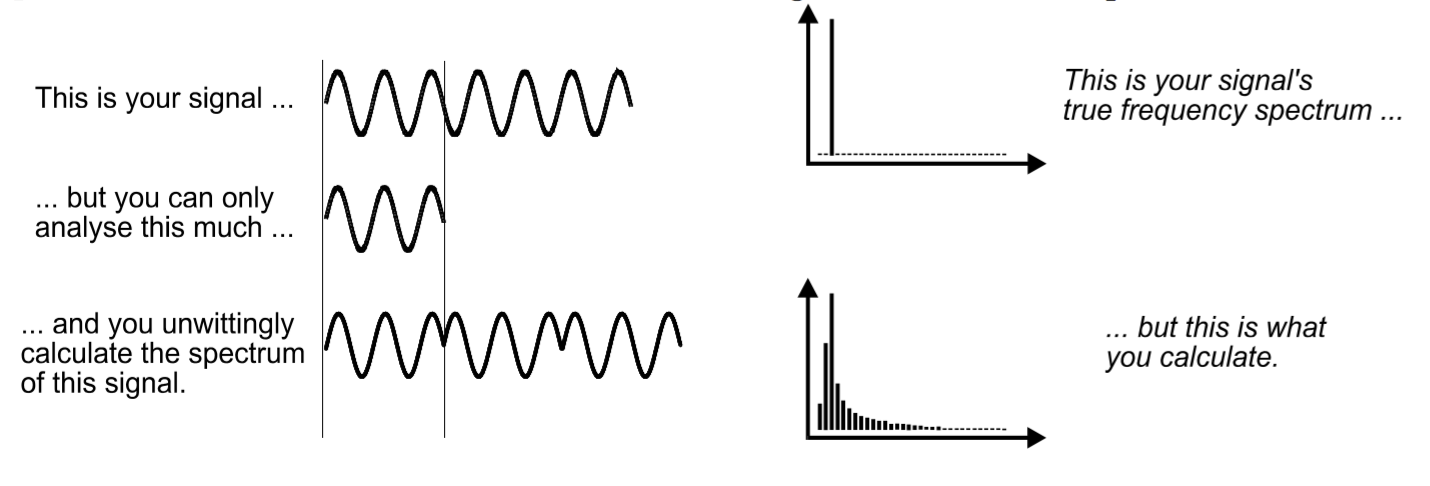
\includegraphics[width=\linewidth]{images/figure_straddleloss.png}	
%	\caption{Three functions with different Amplitudes}
%	\label{fig:leakExplain}
%\end{figure}
%
%\begin{figure}[h!]
%	\centering
%	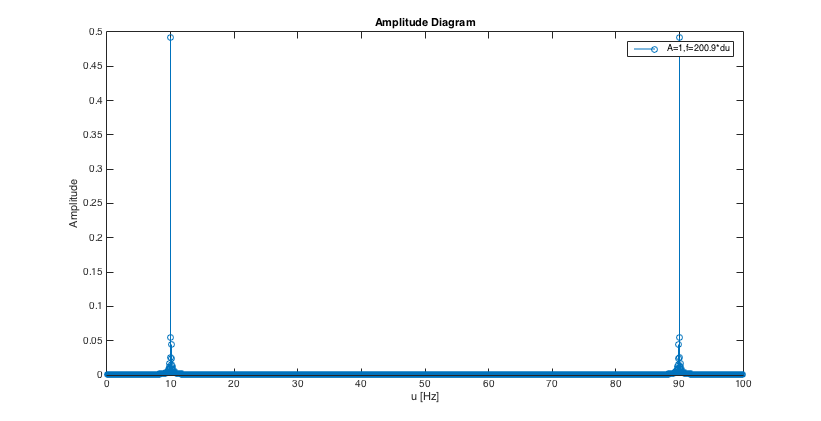
\includegraphics[width=\linewidth]{images/ass1_5}	
%	\caption{Harmonic function with value for C = 200.9}
%	\label{fig:leak}
%\end{figure}

\subsection{Explanation of Leakage}
\begin{figure}[!htbp]
  \centering
  \begin{minipage}[b]{0.9\textwidth}
    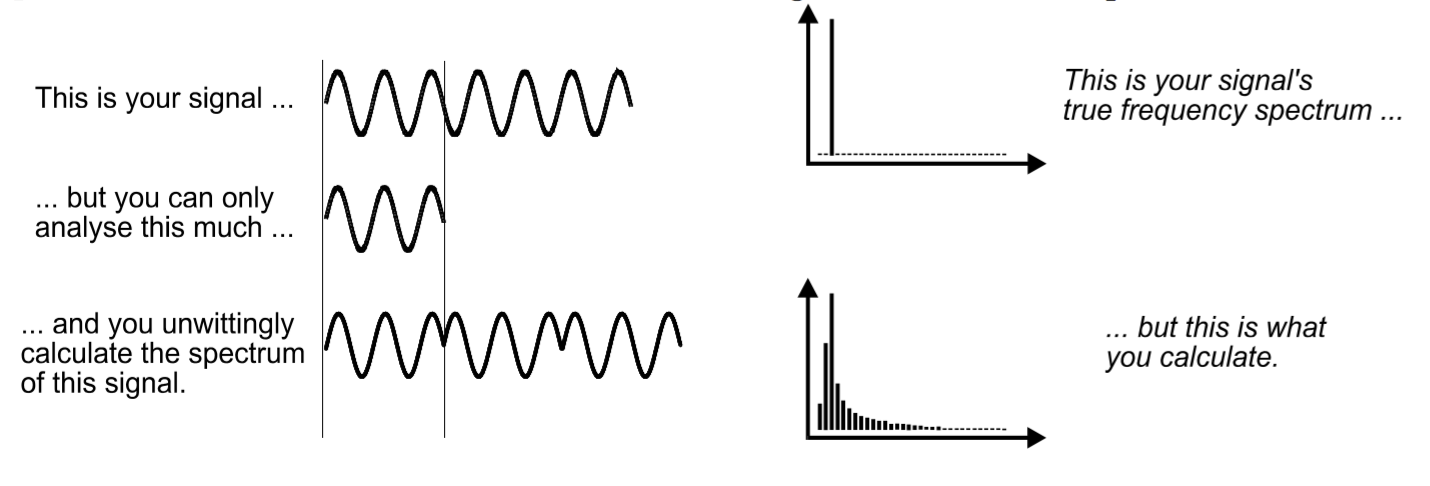
\includegraphics[width=\textwidth]{images/figure_straddleloss}
    \caption{Leakage from truncation, (\textit{Source: Lab Instructions})}
    \label{fig:leakExplain}
  \end{minipage}
  \vfill
  \begin{minipage}[b]{0.9\textwidth}
    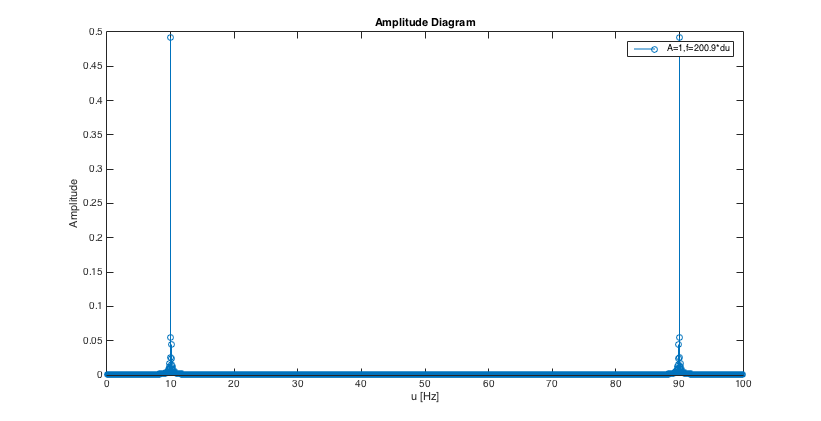
\includegraphics[width=\textwidth]{images/ass1_5}
    \caption{Harmonic function with value for C = 200.9}
    \label{fig:leak}
  \end{minipage}
\end{figure}

The problem that happens, when the truncation does not happen exactly at the period is, that the spectrum becomes "less sharp" (c.f. fig. \ref{fig:leak}), which means that the main peak is accompanied by smaller peaks at the bottom part of the diagram. Also, the main peak is a little bit lower. This phenomenon is called leakage.

\subsection{Straddle Loss}
The problem with leakage for radar signals, is that leakage significantly reduces the Signal-to-Noise-Ratio which makes it "harder" to detect the proper signal, as can be seen in fig. \ref{fig:leak} and fig. \ref{fig:leakExplain}. This is also called "straddle-loss". It is basically a consequence of not appropriate or good enough sampling.

%noise, and bad for radar
%
%b) straddle loss -> significant reduction of SNR
%
%basically consequence of bad sampling


%%%%%%%%%%%%%%%%% TASK 6 %%%
%\section{Phase Diagram}
\addtocounter{section}{1}

%%%%%%%%%%%%%%%%% TASK 7 %%%
%\section{Inverse DFT}
\addtocounter{section}{1}

%%%%%%%%%%%%%%%%% TASK 8 %%%
\section{Rectangular Function}
\label{rect}
Plotting the DFT of the rectangular function

\[ x(t) =
  \begin{cases}
    1       & \quad \text{if }  0 \leq t < 3s \\
    0  		& \quad \text{if }  3s \leq t \\
  \end{cases}
\]
for t $\leq$ 6 with sampling distance of 1 second  shows  the sinc-function (in the frequency domain), but due to the very less given samples the sinc-function is not very clear, means the frequency resolution is quite bad. Also, since the given number of samples is even, the left and right halves of the transform are not "mirrored" at the y-axis but show different peaks (right side one less than left side), see red parts in fig. \ref{fig:mirror}. To increase this frequency resolution a technique called \textit{zeropadding} is applied, see next chapter.

%%%%%%%%%%%%%%%%% TASK 9 %%%
\section{Zeropadding}

\begin{figure}[h!]
	\centering
	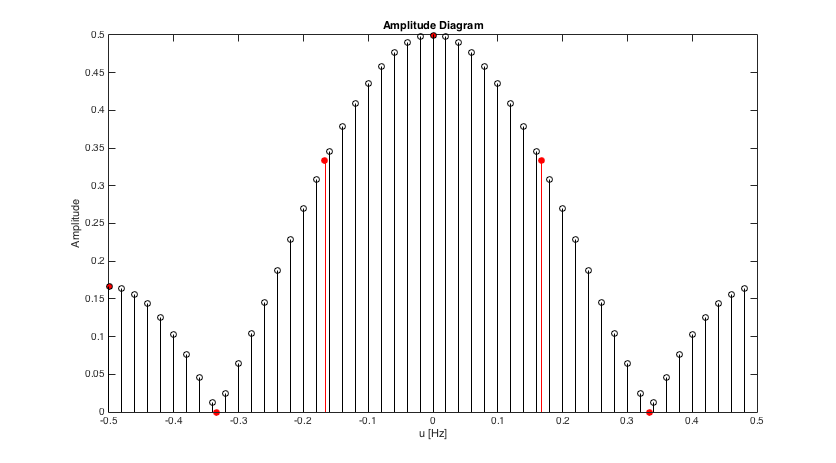
\includegraphics[width=\linewidth]{images/ass1_8_9}	
	\caption{Sinc-function, zeropadded}
	\label{fig:mirror}
\end{figure}

In fig. \ref{fig:mirror} the black peaks represent the zeropadded rectangular function from task \ref{rect}.

\begin{enumerate}[label=\alph*)]
	\item Compared to the main peak lobe, the peak side lobe (Amplitude 0.16) is lower by about 0.33.
	\item Again, reading from fig. \ref{fig:mirror}, the amplitude is reduced by 50\% at a frequency of $\pm$ 0.2 Hz.
	\item Expressing the previous items as 10*log(amplitude) results in: 
	\begin{itemize}
		\item 10 * log(0.33) = -4.81 dB
		\item 10 * log(0.2)  = -3 dB
	\end{itemize}
\end{enumerate}


%%%%%%%%%%%%%%%%% TASK 10 %%%
\section{Dirac’s delta function $\delta$(t)}
The Fourier Transform of a constant function (constant level in the time domain, DC-Level) is the Dirac's delta function in the frequency domain, and vice versa. This is also addressed as the duality of transform pairs.


%%%%%%%%%%%%%%%%% TASK 11 %%%
\section{Sinc Function}

Plotting and varying the values leads to the conclusion, that the broader the function is in time domain, the narrower it is in the frequency domain and vice versa.


%%%%%%%%%%%%%%%%% TASK 12 %%%
\section{Noise, auto correlation and cross correlation}
\subsection{Mean of Many Realizations}

\begin{figure}[h!]
	\centering
	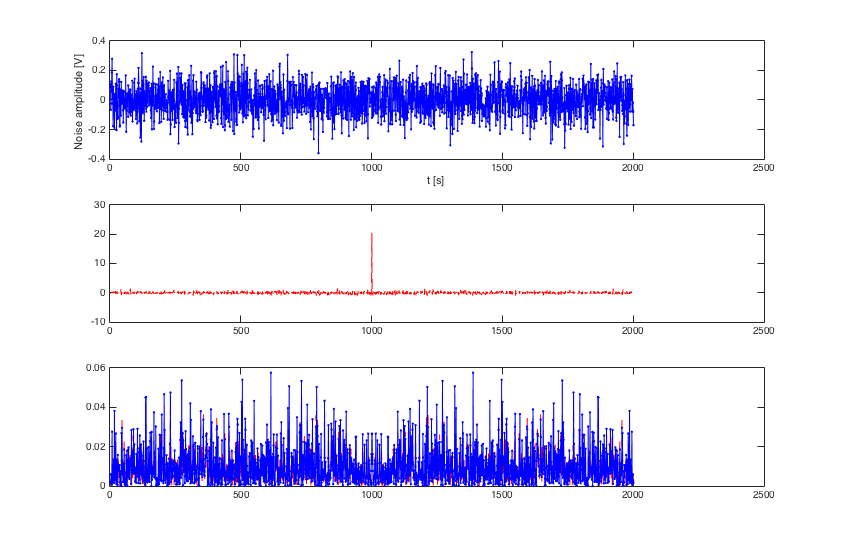
\includegraphics[width=\linewidth]{images/ass1_12}	
	\caption{Noise, Auto-correlation and Power Spectrum}
	\label{fig:12_1}
\end{figure}

Taking the mean of many realization leads to more averaging, and thus to more noise cancellation. Also, the auto correlation peak is standing out more, since one takes multiple realizations.

\subsection{Power spectrum and autocorrelation function}

In the power spectrum graphs the DC component is always visible, with the ideal plot being an exception, the red line in the plotted functions of the provided MATLAB-file \textit{pulseNoise2016.m}. This DC component can not get rid off by simple averaging. Whereas the noise, also always present can be averaged and thus more or less cancelled.

In the autocorrelation functions the noise and DC is also always visible, as well as the cross-correlation triangle, which has features of auto-correlation.


\subsection{Integration in the signal Path}
The auto-correlation function and the power spectrum differs depending on where in the signal path the integration is performed, since one get rid of noise by averaging, which makes it better to apply FFT in the end (after the integration), than for each single sample, where the noise is present and obviously influences the FFT, since it is not cancelled out.

\end{document}
